\documentclass[reqno]{amsart}
\usepackage[utf8]{inputenc}
\usepackage[margin=1in]{geometry}
\usepackage[usenames, dvipsnames]{xcolor}
\usepackage{graphicx}
\usepackage{mathtools}
\usepackage{amssymb}
\usepackage{amsthm}
\usepackage{fancyhdr}
\usepackage{adforn}
\usepackage{xparse}
\usepackage{tikz}
\usetikzlibrary{fadings}
%\usetikzlibrary{matrix, positioning, calc}
% Additional math macros that I want in both my notes and my psets
\usepackage[sc, noBBpl]{mathpazo}
\usepackage{mathrsfs}
\usepackage[T1]{fontenc}
\usepackage{calligra}
\usepackage{microtype}
\usepackage[all]{xy}
\usepackage{slashed}
\newcommand{\A}{\mathbb A}
\newcommand{\cat}{\mathsf}
\newcommand{\sC}{\cat C}
\newcommand{\sD}{\cat D}
\newcommand{\sS}{\cat S}
\newcommand{\sA}{\mathscr A}
\newcommand{\sF}{\mathscr F}
\newcommand{\sG}{\mathscr G}
\renewcommand{\P}{\mathbb P}
\newcommand{\cO}{\mathscr O}
\newcommand{\sI}{\mathscr I}
\DeclareMathOperator{\coker}{coker}
\renewcommand{\Im}{\operatorname{Im}}
\newcommand{\pt}{\mathrm{pt}}
\DeclareMathOperator{\Hom}{Hom}
\newcommand{\op}{^{\mathsf{op}}}
\newcommand{\Id}{\mathrm{Id}}
\DeclareMathOperator{\Mat}{Mat}
\newcommand{\m}{\mathfrak m}
%\newcommand{\p}{\mathfrak p}
\newcommand{\q}{\mathfrak q}
\DeclareMathOperator{\MSpec}{MSpec}
\DeclareMathOperator{\Spec}{Spec}
\newcommand{\Top}{\cat{Top}}
\newcommand{\Ring}{\cat{Ring}}
\newcommand{\Mod}{\cat{Mod}}
\DeclareMathOperator{\res}{res}
\newcommand{\Alg}{\cat{Alg}}
\newcommand{\Fun}{\cat{Fun}}
\newcommand{\AffSch}{\cat{AffSch}}
\newcommand{\Ab}{\cat{Ab}}
\DeclareMathOperator{\bl}{--}
\DeclareMathOperator{\Free}{Free}
\DeclareMathOperator{\For}{For}
\newcommand{\Set}{\cat{Set}}
\newcommand{\LocRing}{\cat{LocRing}}
\newcommand{\Grp}{\cat{Grp}}
\newcommand{\Sch}{\cat{Sch}}
\newcommand{\inHom}{\operatorname{\underline{\Hom}}}
\DeclareMathOperator{\Frac}{Frac}
\DeclareMathOperator{\Gal}{Gal}
\DeclareMathOperator{\Nil}{Nil}
\newcommand{\pre}{\sC^{\text{pre}}}
\newcommand{\sh}{_{\text{sh}}}
\newcommand{\G}{\mathbb G}
\DeclareMathOperator{\Proj}{Proj}
\newcommand{\sM}{\mathscr M}
\newcommand{\sV}{\mathscr V}
\newcommand{\fU}{\mathfrak U}
\newcommand{\GL}{\mathrm{GL}}
\DeclareMathOperator{\Sym}{Sym}
% http://tex.stackexchange.com/questions/141434/how-to-type-sheaf-hom
\DeclareMathOperator{\shom}{\mathscr{H}\text{\kern -4pt {\calligra\large om}}\,}
\newcommand{\sL}{\mathscr L}
\DeclareMathOperator{\QC}{QC}
\DeclareMathOperator{\Supp}{Supp}
\newcommand{\sN}{\mathscr N}
\DeclareMathOperator{\Ann}{Ann}
\DeclareMathOperator{\Der}{Der}
\newcommand{\ctcpx}[1]{(#1)^{\text{der}}}
\newcommand{\Dist}{\mathsf{Dist}}
\newcommand{\shdi}{\operatorname{Sh}_{\Dist}}
\DeclareMathOperator{\Sh}{Sh}
\newcommand{\shz}{\mathsf{Sh}_{\text{\rm Zar}}}
\DeclareMathOperator{\Gr}{Gr}
% Source: http://tug.org/pipermail/xy-pic/2001-July/000015.html
\newcommand{\pullbackcorner}[1][dr]{\save*!/#1+1.2pc/#1:(1,-1)@^{|-}\restore}
\newcommand{\pushoutcorner}[1][dr]{\save*!/#1-1.2pc/#1:(-1,1)@^{|-}\restore}
\newcommand{\TDel}{\mathrm{2\Delta}}
\DeclareMathOperator{\Bl}{B\ell}
\newcommand{\cR}{\mathcal R}
\newcommand{\cL}{\mathcal L}
\newcommand{\cH}{\mathcal H}
\newcommand{\refR}{\reflectbox{\(\cR\)}}

\renewcommand{\a}{\alpha}
\renewcommand{\b}{\beta}
%\newcommand{\e}{\epsilon}
\renewcommand{\l}{\lambda}
\renewcommand{\L}{\Lambda}
\newcommand{\g}{\gamma}
\newcommand{\s}{\sigma}
\newcommand{\z}{\zeta}
\newcommand{\RR}{\mathbb{R}}
\newcommand{\NN}{\mathbb{N}}
\newcommand{\QQ}{\mathbb{Q}}
\newcommand{\ZZ}{\mathbb{Z}}
\newcommand{\CC}{\mathbb{C}}
\newcommand{\cC}{\mathcal{C}}
\newcommand{\f}{\frac}
\newcommand{\p}{\partial}
\renewcommand{\P}[3][]{\f{\partial^{#1} #2}{\partial #3 ^{#1}}}
%\newcommand{\avg}[1]{\langle #1 \rangle}
\newcommand{\avg}[1]{\left< #1 \right>}
\newcommand{\?}{\overset{?}{=}}
\newcommand{\Int}{\int_{-\infty}^\infty}
\newcommand{\ket}[1]{\left| #1 \right>} % for Dirac bras
\newcommand{\bra}[1]{\left< #1 \right|} % for Dirac kets
\newcommand{\braket}[2]{\left< #1 \vphantom{#2} \right|
 \left. #2 \vphantom{#1} \right>} % for Dirac brackets
\newcommand{\pv}{\vec{p}}

\newcommand{\grad}[1]{\gv{\nabla} #1} % for gradient
\let\divsymb=\div % rename builtin command \div to \divsymb
\renewcommand{\div}[1]{\gv{\nabla} \cdot #1} % for divergence
\newcommand{\curl}[1]{\gv{\nabla} \times #1} % for curl
\renewcommand{\labelenumi}{(\alph{enumi})}
\let\vaccent=\v % rename builtin command \v{} to \vaccent{}
\renewcommand{\v}[1]{\ensuremath{\mathbf{#1}}}
\newcommand{\uv}[1]{\ensuremath{\mathbf{\hat{#1}}}} % for unit vector
\newcommand{\gv}[1]{\ensuremath{\mbox{\boldmath$ #1 $}}} 
% for vectors of Greek letters
\usepackage{hyperref}
\usepackage{siunitx}

%\usepackage[compat=1.1.0]{tikz-feynman}

% TODO fiddle with colors
\definecolor{newblue}{HTML}{1F98A6}
\definecolor{newred}{HTML}{D95448}
\definecolor{neworange}{HTML}{F29441}
\hypersetup{
	colorlinks,
	linkcolor=newred,
	citecolor=neworange,
	urlcolor=newblue!80!black,
}
\usepackage[all]{hypcap}
\pagestyle{plain}
\setcounter{tocdepth}{1}


\usepackage{titlesec}
\titleformat{\section}[frame]
  {\normalfont}
  {\filright
   \footnotesize
   \enspace Lecture \arabic{section}.\enspace}
  {8pt}
  {\Large\bfseries\filcenter}
\usepackage[dotinlabels]{titletoc}
\titlecontents{section}[1.5em]{}{\contentslabel{2.3em}}{\hspace*{-2.3em}}{\hfill\contentspage}

\renewcommand{\sectionmark}[1]{\markleft\thesection. #1}

\fancyhf{}
\fancyhead[RO,LE]{\small\thepage}
\fancyhead[LO]{\small\slshape\nouppercase{\rightmark}}
\fancyhead[RE]{\small\slshape Advanced Quantum Field Theory Lecture Notes}
\setlength{\headheight}{11.0pt}
\pagestyle{fancy}

\numberwithin{equation}{section}
\newcommand{\orbreak}{
\begin{center}
	\adforn{17}\;\(\cdot\)\;\adforn{18}
	\vspace{0.2cm}
\end{center}
}

\renewcommand{\labelitemi}{\(\circ\)}

% I wanted to allow one to reference parts of a thm/cor/etc. and have it print the thm number too, e.g. 29.2(1),
% but this isn't working right now. Probably the best way to do this would be to play around with enumitem to
% define a new enumerate-like counter and then just use that directly instead of enumerate in comp.

% This feels really wobbly, but so far it's working
\NewDocumentEnvironment{comp}{mm}{%
	\csname #1\endcsname\hfill
	\csname #2\endcsname
}{
	\csname end#2\endcsname
	\csname end#1\endcsname
}

% usage:
% \shortexact[f][g]{A}{B}{C},
%
%			 f    g
% for 0 -> A -> B -> C -> 0,
\DeclareDocumentCommand{\shortexact}{O{} O{} mmmm}{
\xymatrix{
	0\ar[r] & #3\ar[r]^-{#1} & #4\ar[r]^-{#2} & #5\ar[r] & 0#6
}}
% exactly the same, but for 0 -> A -> B -> C
\DeclareDocumentCommand{\leftexact}{O{} O{} mmmm}{
\xymatrix{
	0\ar[r] & #3\ar[r]^-{#1} & #4\ar[r]^-{#2} & #5 #6
}}
% ... and the same, for A -> B -> C -> 0
\DeclareDocumentCommand{\rightexact}{O{} O{} mmmm}{
\xymatrix{
	#3\ar[r]^-{#1} & #4\ar[r]^-{#2} & #5\ar[r] & 0#6
}}



% usage:
% X\dblarrow[r] & Y
%   f
% X => Y
%   g
\DeclareDocumentCommand{\dblarrow}{O{} O{} O{}}{
	\ar@<0.4ex>[#1]^-{#2}\ar@<-0.4ex>[#1]_-{#3}
}
% Note: it would be a useful exercise to figure out how to define this so it can be used as
% \dblarrow[r]^f_g

\everyentry={\displaystyle}

\newcommand{\N}{\mathbb N}
\newcommand{\Z}{\mathbb Z}
\newcommand{\Q}{\mathbb Q}
\newcommand{\R}{\mathbb R}
\newcommand{\C}{\mathbb C}
\newcommand{\F}{\mathbb F}
\newcommand{\vp}{\varphi}
\newcommand{\term}{\emph}
\renewcommand{\vec}[1]{\boldsymbol{\mathbf{#1}}}
\DeclarePairedDelimiter\paren{(}{)}
%\DeclarePairedDelimiter\ang{\langle}{\rangle}
\DeclarePairedDelimiter\abs{\lvert}{\rvert}
\DeclarePairedDelimiter\norm{\lVert}{\rVert}
\DeclarePairedDelimiter\bkt{[}{]}
\DeclarePairedDelimiter\set{\{}{\}}
% Swap paren* and paren, etc., so that the normal version resizes by default.
% Meanwhile, one can use \paren*[\Big]{...} to customize the size easily.
% It would be interesting to wrap this up into a custom \definedelimiter command...
\makeatletter
	\let\oldparen\paren
	\def\paren{\@ifstar{\oldparen}{\oldparen*}}
	\let\oldbkt\bkt
	\def\bkt{\@ifstar{\oldbkt}{\oldbkt*}}
\makeatother
\newcommand{\e}{\varepsilon}
\def\qedsymbol{{\small{\ensuremath{\boxtimes}}}}
\newcommand{\inj}{\hookrightarrow}
\newcommand{\surj}{\twoheadrightarrow}
\DeclareMathOperator{\id}{id}
\newcommand{\ud}{\,\mathrm{d}}
\renewcommand{\d}{\mathrm d}
\newcommand{\dfr}[2]{\frac{\mathrm d #1}{\mathrm d #2}}
\newcommand{\pfr}[2]{\frac{\partial #1}{\partial #2}}

%\catcode`\"=13
%\newcommand{"}[1]{^{(#1)}}
\newtheorem{thm}[equation]{Theorem}
\newtheorem*{thm*}{Theorem}
\newtheorem{lem}[equation]{Lemma}
\newtheorem*{lem*}{Lemma}
\newtheorem{cor}[equation]{Corollary}
\newtheorem{prop}[equation]{Proposition}
\newtheorem{obs}[equation]{Observation}
\theoremstyle{definition}
\newtheorem{ex}[equation]{Exercise}
\newtheorem{exm}[equation]{Example}
\newtheorem{defn}[equation]{Definition}
\newtheorem*{claim}{Claim}
\theoremstyle{remark}
\newtheorem*{rem}{Remark}
\newtheorem*{fct}{Fact}
\newtheorem*{note}{Note}

\begin{document}
\title{Black Holes}
\author{Ian Lim\\ Last updated \today}
\maketitle
{\small\noindent These notes were taken for the \textit{Black Holes} course taught by Jorge Santos at the University of Cambridge as part of the Mathematical Tripos Part III in Michaelmas Term 2018. I live-\TeX ed them using Overleaf, and as such there may be typos; please send questions, comments, complaints, and corrections to 
\href{mailto:itel2@cam.ac.uk?subject=BH\%20Lecture\%20Notes}{\texttt{itel2@cam.ac.uk}}.\\
Many thanks to Arun Debray for the {\LaTeX} template for these lecture notes: as of the time of writing, you can find him at \url{https://web.ma.utexas.edu/users/a.debray/}.}

\tableofcontents

\section{Friday, January 18, 2019}
	\begin{note}
    Here's the relevant admin content for the first day. The lecturer's email is \url{n.datta@damtp.cam.ac.uk}., and course notes can be found on the CQIF webiste under Part III lectures.
\end{note}

Quantum information theory (QIT) was born out of classical information theory (CIT).
\begin{defn}
Classical information theory is the mathematical theory of information processing tasks, e.g. storage, transmission, processing of information.
\end{defn}
In contrast, quantum information theory asks how these tasks can be performed if we harness quantum mechanical systems as information carriers. Such systems include electrons, photons, ions, etc.

QM has some novel features which are not present in our old Newtonian theories. We know that quantum systems obey the Heisenberg uncertainty principle, that energy is quantized in these systems, and QM systems cannot generically be copied (the famous no-cloning theorem).
Quantum mechanically, one can describe the full state of a system without knowing the state of the subsystems-- this is essentially the idea of entanglement.%
    \footnote{If you like, some composite states in a tensor product space cannot be decomposed into a direct product.}

Here's a quick overview now of the structure of the course.
\begin{itemize}
    \item Basic concepts of CIT
    \item Study of open quantum systems
    \item Mathematical tools for QIT
    \item Entanglement
    \item QIT itself
\end{itemize}
When we say open quantum systems, we mean quantum systems which interact with a broader environment. If we prepare a state and allow it to interact, what happens to the information stored in that state?

\subsection*{Classical information theory} Historically, CIT was invented in 1948 with a pioneering paper by Claude Shannon. In this paper, he asked two critical questions.
\begin{itemize}
    \item[Q1.] What is the limit to which information can be \emph{reliably} compressed?
    \item[Q2.] What is the maximum rate at which information can be reliably sent through a communication channel?
\end{itemize}
That is, we may ask about how to encode information in such a way that it can still be recovered with a high probability of success. And we can ask how to send this information when our communication channels will naturally be noisy. The answers to these questions are known as \term{Shannon's Source Coding Theorem} and \term{Shannon's Noisy Channel Coding Theorem}, respectively.

\subsection*{What is information?} We have an intuitive sense of what information means, but to formalize this takes a little work. In the loosest sense, information is associated to uncertainty and in particular information gain is related to a reduction in uncertainty.
\begin{exm}
Suppose I have a system which takes some discrete values, e.g. I roll a fair die. The outcome is a variable $x$ which takes values in some set, $J=\set{1,2,\ldots, 6}$. We write that capital $X$ is proportional to $p(x),x\in J$, where $P(X=x)=p(x)=1/6\, \forall x\in J$. That is, there is a probability mass function associated to the possible outcomes. The probability that we measure the system $X$ in outcome $x$ is $1/6$ for any outcome $x$ in the set of outcomes.
\end{exm}

We also define the following quantity.
\begin{defn}
\term{Surprisal} is the quantity
\begin{equation}
    \gamma(x)=-\log p(x).
\end{equation}
When an event is very unlikely and it happens anyway... you are very surprised. For example, $p(x)=1\implies \gamma(x)=0$ (certainties are not very surprising) while $p(x)\approx 0 \implies \gamma(x)$ large.
\end{defn}
This quantity has some features:
\begin{itemize}
    \item It only depends on $p(x)$ and not on $x$.
    \item It is a continuous function of $p(x).$
    \item It is additive for independent events.
\end{itemize}
This last property is easy to prove:
\begin{equation*}
    P(X=x,Y=y)=P_{XY}(x,y)=P_X(x)P_Y(y)
\end{equation*}
when $X,Y$ are independent. Then
\begin{equation*}
    \gamma(x,y)=-\log P_{XY}(x,y)=\gamma(x)+\gamma(y).
\end{equation*}

\begin{defn}
    We can now define the \term{Shannon entropy} of $X$ to be
    \begin{equation}
        H(X)\equiv \mathbb{E}(\gamma(X))=\sum_{x\in J}(-\log(p(x))p(x),
    \end{equation}
    the expected value of the surprisal. We see again that $H(X)$ does not depend on the actual outcomes themselves but only on the probability distribution $P(X)$.
\end{defn}
As a matter of convention we will take logs to be $\log{} \equiv \log_2{}$, and for events which are impossible $P(x)=0$ we have $0\log 0 = 0$ (which one can prove by taking the limit $\lim_{u\to 0}u\log u =0.$

\subsection*{Binary entropy} Consider an event which has two possible outcomes, $X\sim P(x), x\in J =\set{0,1}$ where $P(X=0)=p$ and $P(X=1)=1-p$. Then the Shannon entropy is
\begin{equation}
    H(X)=-p\log p - (1-p)\log(1-p)\equiv h(p).
\end{equation}
We see that if the probability is $p=1/2$, then we have no information a priori about this systems-- the entropy is maximized. $h(p)$ is a continuous function of $P$, and it is concave.

\begin{defn}
    We can also define a different entropy, the Renyi entropy, which is
    \begin{equation}
        H_\alpha(X)=\frac{1-\alpha}\log (\sum_{x\in J}P(x)^\alpha),
    \end{equation}
    with $\alpha \in (1,2]$. As an exercise, we can verify that $\lim_{\alpha \to 1} H_\alpha(X) = H(X)$, i.e. the Renyi entropy reduces to the Shannon entropy.
\end{defn}

Why do we choose to work with the Shannon entropy? It has to do with the operational interpretation-- the Shannon entropy represents an optimal rate of data compression, i.e. the data compression limit.

In CIT, a classical information source emits some messages/data/signals/information. For instance, $J$ could output a binary output or perhaps telegraph English (26 letters and a space). Now, the simplest class of sources is \term{memoryless}-- they are ``independent identically distributed'' sources (i.i.d.), which means that successive messages are independent of each other, and they are identically distributed.

\begin{defn}
    Suppose we have some random variables $U_1,U_2,\ldots, U_n$ with $U_i \sim p(u),u\in J$. We say these are \term{identically distributed} if
    \begin{equation*}
        p(u)=P(U_k=u), u\in J \quad \forall 1\leq k \leq n.
    \end{equation*}
\end{defn}
We could study a signal emitted by $n$ uses of the source to get some sequence $\underline{u}^{(n)}=(u_1,u_2,\ldots, u_n)$.
\begin{defn}
    Moreover, if the probability mass function takes the form
    \begin{align*}
        p(\underline{u^{(n)}}) &=P(U_1,\ldots,U_n= u_n)\\
        &= p(u_1)\ldots p(u_n).
    \end{align*}
\end{defn}

If the source is indeed independent and identically distributed, then it makes sense to describe it by a sincle probability mass function, $U\sim p(u)$, so that the Shannon entropy of the source can be siad to be
\begin{equation}
    H(U)=-\sum_{u\in J} p(u) \log p(u).
\end{equation}

Another guiding question. Why is data compression possible? Our information source has some \emph{redundancy}. For instance, in the English language, certain letters are more common than others, so we can encode something that is more common in a shorter string in anticipation it will be used more often.

This sort of scheme is known as variable length coding, e.g. we might encode the letter ``e'' as the string $10$ and the letter ``z'' as $11000$. In contrast, we could also use a fixed length coding scheme where we have a ``typical set'', a subset of our total outcomes $J^n$ (things we might like to encode). Our typical set then has a one-to-one mapping to the set of encoded messages, e.g. $\set{0,1}^m$, so we can always recover them precisely, while several outcomes outside the typical set might map to the same encoded message. There's some probability that we'll want to encode things outside the typical set, and in decoding we'll get the original message a little bit wrong. But if we choose the typical set well, this can be made to be a rare occurrence. We are usually interested in \emph{asymptotic i.i.d.} settings, i.e. in the limit as the size of the set of possible messages to be encoded goes to $\infty$.

\begin{exm}
    Suppose we have a horse race with eight horses. They have labels $1,2\ldots, 8$, and the message we would like to encode is the label of the winning horse. A priori, we only need $3$ bits to encode the label since $2^n$ different messages can be stored in $n$ bits.
    
    However, what if the horses are of different abilities? Realistically, they won't all be equally fast. Suppose that $p_i$ is the probability of the $i$th horse winning, such that
    \begin{equation*}
        p_i=1/2,1/4,1/8,1/16,1/64,\ldots,1/64.
    \end{equation*}
    Now we assign the following code words:
    \begin{align*}
        C(1)&=0\\
        C(2)&=10\\
        C(3)&=110\\
        C(4)&=1110\\
        C(5)&=111100\\
        C(6)&=111101\\
        \vdots&
    \end{align*}
    Let $l_i$ be the length of the $i$th codeword, e.g. $l_5=6$. We can show that the average length of a code is then $\sum p_i l_i = 2$, and we've chosen a prefix-free code so that e.g. a sequence like 10011001110 can be uniquely decoded to a sequence of winners from our code words.
\end{exm}

\section{Monday, January 21, 2019}
    Last time, we introduced a \term{worldline action} with an einbein $e$ (auxiliary field).
\begin{equation*}
    S[x,e]=\frac{1}{2}\int d\tau \left(e^{-1} \eta_{\mu\nu} \dot x^\mu \dot x^\nu-e m^2\right).
\end{equation*}
In the massless limit, this reduces to
\begin{equation}
    S[X,e]=\frac{1}{2} d\tau e^{-1} g_{\mu\nu} \dot x^\mu \dot x^\nu,
\end{equation}
where we have replaced the Minkowski metric with some generic metric. The classical equations of motion for $X^\mu(\tau)$ then give the geodesic equation,
\begin{equation}
    \ddot X^\mu +\Gamma^\mu_{\nu\lambda} \dot X^\nu \dot X^\lambda = 0.
\end{equation}
The $e(\tau)$ equations of motion would give some constraints. However, if we attempted to quantize this theory, we would find that the background metric $g_{\mu\nu}$ is not actually deformed in the solutions. Rather than being dynamic as in general relativity, it's sort of a thing that is given to us and sits in the background, unchanging, which is why for a particle this is not a theory of quantum gravity. As we'll see, this is \emph{not} the case for strings.

\subsection*{Strings} As a string moves through some flat spacetime $\cM$ with metric $\eta_{\mu\nu}$, it sweeps out a worldsheet $\Sigma.$ Assume that the string is closed, so it has a coordinate $\sigma$ (along the length of the string, if you like):
\begin{equation*}
    \sigma \sim \sigma + 2n\pi, n\in \ZZ.
\end{equation*}
And it moves through time as parametrized by a proper time $\tau$, so the embedding of the worldsheet is given by $X^\mu(\sigma,\tau)$. That is, $\sigma$ and $\tau$ provide good coordinates for the worldsheet in $\cM$.
\begin{defn}
    We call these $X^\mu$ embedding fields. They are maps
    $X:\Sigma \to \cM$ from the worldsheet to the background spacetime manifold.
\end{defn}
We also say that the area of the worldsheet $\Sigma$ is given by
\begin{equation}
    \text{area}=\int d\tau d\sigma \sqrt{-\det(\eta_{\mu\nu} \p_a X^\mu \p_0 X^\nu)}
\end{equation}
where $\sigma^a =(\tau, \sigma)$ so that $\p_a = \P{}{\sigma^a}.$ In fact, we shall introduce an extra factor know (for historical reasons) as $\alpha'$ and write
\begin{equation}\label{nambugoto}
    S[X]=-\frac{1}{2\pi \alpha'}\int d\tau d\sigma \sqrt{-\det(\eta_{\mu\nu} \p_a X^\mu \p_b X^\nu)},
\end{equation}
where $\alpha'$ is a free parameter. We often refer to the \term{string length},
\begin{equation}
    l_s \equiv 2\pi\sqrt{\alpha'}
\end{equation}
or the \term{tension}
\begin{equation}
    T \equiv \frac{1}{2\pi \alpha'}.
\end{equation}

\begin{defn}
    The object
    \begin{equation}
        G_{ab}\equiv \eta_{\mu\nu} \p_a X^\mu \p_b X^\nu
    \end{equation}
    is an induced metric on $\Sigma$, and the action \ref{nambugoto} is called the \term{Nambu-Goto action}.
\end{defn}
Having just defined this, we won't really do anything with it for the rest of the course. Bummer. However, to make up for it, let's write down a new and improved action, the \term{Polyakov action}.

\begin{defn}
    Consider the action
    \begin{equation}\label{polyakovaction}
        S[X,h]=-\frac{1}{4\pi \alpha'} \int_\Sigma d^2\sigma \sqrt{-h}\,h^{ab} \eta_{\mu\nu} \p_a X^\mu \p_b X^\nu.
    \end{equation}
    This should remind us of what we did with the einbein last lecture, where we introduced $e$ into our action.
    
    This \term{Polyakov action} is classically equivalent to the Nambu-Goto action, since this auxiliary $h$ which we have introduced will turn out to be non-dynamical.
\end{defn}

The $h_{ab}$ equations of motion are given by a weird variation of the action,
\begin{equation}
    -\frac{2\pi}{\sqrt{-h}}\frac{\delta S}{\delta h^{ab}}=0.
\end{equation}
These equations of motion give the vanishing of the stress tensor, $T_{ab}=0$, where
\begin{equation}
    T_{ab}=-\frac{1}{\alpha'}\paren{\p_a X^\mu \p_b X_\mu - \frac{1}{2} h_{ab} \p_c X^\mu \p_d X_\mu h^{cd}}.
\end{equation}

Note that in two dimensions, $T_{ab}h^{ab}=0$, i.e. $T_{ab}$ is traceless. This is our first indication that something is different about two dimensions.

The $X^\mu$ equations of motion are
\begin{equation}
    \frac{1}{\sqrt{-h}}(\p_a \sqrt{-h}\, h^{ab} \p_b X^\mu)=0, \quad
    \Box X^\mu =0.
\end{equation}
Now we could imagine adding a cosmological constant (which would cause the trace of the stress tensor to change) or perhaps some sort of Einstein-Hilbert term to our metric $h_{ab}$. But we'll see why this might be more complicated than it initially seems.

\subsection*{Symmetries} The Polyakov action \ref{polyakovaction} has the following symmetries:
\begin{itemize}
    \item Rigid (global) symmetry, $X^\mu(\sigma,\tau)\to \Lambda^\mu{}_\nu X^\nu(\sigma,\tau) + a^\mu$ (Poincar\'e invariance).
    \item Local symmetries-- the physics should be invariant under reparametrizations of the coordinates of the worldsheet, so under transformations $\sigma^a \to \sigma'{}^a (\sigma,\tau).$ The fields themselves transform as
    \begin{align*}
        X'^\mu(\sigma',\tau')&= X^\mu(\sigma,\tau)\\
        h_{ab}(\sigma,\tau)&= \P{\sigma'{}^c}{\sigma^a} \P{\sigma'{}^d}{\sigma^b} h'_{cd}(\sigma',\tau').
    \end{align*}
    Infinitesimallly, this means that $\sigma^a \to \sigma^a - \xi^a(\sigma,\tau)$, which gives us the variations
    \begin{align*}
        \delta X^\mu &= \xi^a \p_a X^\mu\\
        \delta h_{ab} &= \xi^c \p_c h_{ab}+\p_a \xi^c h_{cb} +\p_b \xi^c h_{ca} =\nabla_a \xi_b +\nabla_b \xi_a\\
        \delta \sqrt{-h} &=\p_a(\xi^a \sqrt{-h}).
    \end{align*}
    Note this second variation, $\delta h_{ab}$, can be written in terms of some covariant derivatives for an appropriate connection, but we won't usually bother.
    \item Weyl transformations-- we send
    \begin{align*}
        X'{}^\mu (\sigma,\tau) &= X^\mu(\sigma, \tau)\\
        h'_{ab}(\sigma,\tau)&=e^{2\Lambda(\sigma,\tau)}h_{ab}(\sigma,\tau).
    \end{align*}
    Thus $\delta X^\mu=0$ and $\delta h_{ab}=2\Lambda h_{ab}$.
    Under such transformations, we have three arbitrary degrees of freedom in $(\xi^a,\Lambda)$ (two from the two components of $\xi$ plus one from $\Lambda$), and we can use them to fix the three degrees of freedom in $h_{ab}$ (there are three, since $h$ is symmetric and $2\times 2$).
\end{itemize}

\subsection*{Classical solutions} Let us now use reparametrization invariance to fix
\begin{equation}
    h_{ab}=e^{2\phi} \eta_{ab}, \quad \eta_{ab}=\begin{pmatrix}
    -1 & 0\\
    0 & 1
    \end{pmatrix}.
\end{equation}
The Polyakov action then becomes
\begin{equation}
    S[X]=-\frac{1}{4\pi \alpha'} \int_\Sigma d^2 \sigma(-\dot X^2 + X'{}^2),
\end{equation}
where
\begin{equation}
    \dot X^\mu \equiv \P{X^\mu}{\tau},\quad X'{}^\mu \equiv \P{X^\mu}{\sigma}
\end{equation}
and squares are taken by contracting with the metric $h_{ab}$. In that case, the $X^\mu(\sigma,\tau)$ equation of motion becomes the wave equation in 2D, %check this?
so solutions are of the form
\begin{equation}
    X^\mu(\sigma,\tau)= X^\mu_R (\tau-\sigma)+X^\mu_L(\tau + \sigma).
\end{equation}
Moreover, since we have a wave equation it is useful to introduce modes $(\alpha^\mu_n, \bar \alpha^\mu_n)$ where
\begin{equation}
    X^\mu_R(\tau-\sigma)=\frac{1}{2}x^\mu +\frac{\alpha'}{2}p^\mu(\tau-\sigma) +i\sqrt{\frac{\alpha'}{2}}\sum_{n\neq 0} \frac{1}{n}
    \alpha^\mu_n e^{-in(\tau-\sigma)},
\end{equation}
where $x^\mu, p^\mu$ are some constants in $(\tau,\sigma)$ and  similarly the left-going modes are
\begin{equation}
    X^\mu_L(\tau+\sigma)=\frac{1}{2}x^\mu +\frac{\alpha'}{2}p^\mu(\tau+\sigma) +i\sqrt{\frac{\alpha'}{2}}\sum_{n\neq 0} \frac{1}{n}
    \bar\alpha^\mu_n e^{-in(\tau+\sigma)}.
\end{equation}
It's sometimes useful to define a zero-mode,
\begin{equation}
    \alpha_0^\mu = \bar \alpha_0^\mu = \sqrt{\frac{\alpha'}{2}}p^\mu.
\end{equation}

\section{Wednesday, January 23, 2019}
    Let's recall the statement of Shannon's source coding theorem. Shannon tells us that if we have an iid source $U\sim p(u); u\in J$ with Shannon entropy $H(U)$, then there is a fundamental limit on data compression given by $H(U)$ such that for any rate $R>H(U)$, there exists a reliable compression-decompression scheme of rate $R,$ and conversely for any rate $R<H(U)$, any scheme of rate $R$ will not be reliable.

See my notes from last lecture for a heuristic argument of the converse. The formal argument can be made with $\epsilon$s and $\delta$s-- for example, my statement that we need not consider elements in $A_\epsilon^{(n)}$ is equivalent to $\sum_{\underline{u}^{(n)}\in S^n \cap A_\epsilon^n} p(\underline{u}^{(n)}) \leq P(A_\epsilon^n \to 0$.

\subsection*{Entropies} Consider a pair of random variables $X,Y$ with \term{joint probability}
\begin{equation}
    P(X=x,Y=y)=P_{XY}(x,y)=p(x,y).
\end{equation}
Here, $x\in J_X$ some alphabet and similarly $y\in J_Y$. We can also define the conditional probability
\begin{equation}
    P(Y=y|X=x)=p(y|x),
\end{equation}
the probability of $y$ given $x$.

\begin{defn}
    Now we have the \term{joint entropy}, which is
    \begin{equation}
        H(X,Y)\equiv -\sum_{x\in J_X,y\in J_Y} p(x,y)\log p(x,y).
    \end{equation}
\end{defn}
\begin{defn}
    We also have the \term{conditional entropy}, which is
    \begin{align*}
        H(Y|X) &\equiv \sum_x p(x) H(Y|X=x)\\
        &= -\sum_x p(x) \sum_y p(y|x) \log p(y|x).
    \end{align*}
\end{defn}
But we can simplify this to write
\begin{equation}
    H(Y|X)=-\sum p(x,y) \log p(y|x),
\end{equation}
which implies that
\begin{equation}
    p(x,y)= p(x) p(y|x) = p(y)p(x|y).
\end{equation}
This leads us to a chain rule,
\begin{equation}
    H(X,Y)= H(Y|X) + H(X).
\end{equation}

We also have the notion of a relative entropy, which measures a ``distance'' between two probability distributions. Suppose we have distributions $p=\set{p(x)}_{x\in J}$ and $q=\set{q(x)}_x\in J$, Let us assume that the $\text{supp}p \subseteq \text{supp} q$, with $\text{supp} p = \set{x\in J: p(x) >0}$. This implies that $q(x)=0\implies p(x)=0$, which we denote $p\ll q$.
\begin{defn}
    Thus we define the \term{relative entropy} to be
    \begin{equation}
        D(p||q)  \equiv \sum_{x\in J} p(x) \log \frac{p(x)}{q(x)}.
    \end{equation}
    If $p\ll q$, then this is well-defined (otherwise we might have $q\to 0$ with $p$ nonzero). Taking $0\log \frac{0}{q(x)}=0$ we see that this represents a sort of distance,
    \begin{equation}
        D(p||q) \geq 0
    \end{equation}
    with equality iff $p=q$.
\end{defn}
This is not quite a true metric, since it is not symmetric, $D(p||q)\neq D(q||p)$, and moreover it does not satisfy a triangle inequality, i.e. $D(p||r)\not\leq D(p||q) +D(q||r)$.

Using the relative entropy, we can now define a useful quantity known as the mutual information.
\begin{defn}
    The mutual information between two sources $X$ and $Y$ is
    \begin{align*}
        I(X;Y) &= H(X)+ H(Y) - H(X,Y)\\
        &= H(X)- H(X|Y).
    \end{align*}
\end{defn}
The mutual information has some intuitive properties.
\begin{itemize}
    \item $I(X:X)=H(X)$, since $I(X;X)=H(X)+H(X)-H(X,X)= H(X)$.
    \item $I(X;Y) = I(Y;X)$
    \item if $X,Y$ independent, then $I(X;Y)=0$.
\end{itemize}

Suppose now we have $P,Q$ taking non-negative real values, with $Q(x)=0 \implies P(X)=0$. THus the relative entropy is
\begin{equation*}
    D(P||Q)=\sum P(x) \log \frac{P(x)}{Q(x)}.
\end{equation*}
What if $P(x)=p(x), x\in J$ and $Q(x)=1 \forall x \in J$? Then
\begin{equation}
    D(P||Q)=\sum_x p(x) \log p(x) = -H(X).
\end{equation}
It's almost trivial to check that if $Q(x)=\frac{1}{|J|}$ instead, then we would get an additional factor of $-\log |J|.$

\begin{ex}
Check that the mutual information satisfies
\begin{equation}
    I(X;Y)=D(p(x,y)|| p(x) p(y)).
\end{equation}
\end{ex}

Let's take a minute to prove the non-negativity of the relative entropy. That is, $D(p||q) \geq 0$.
\begin{proof}
By definition,
\begin{equation}
    D(p||q) = \sum_{x\in J}p(x) \log\frac{p(x)}{q(x)}.
\end{equation}
Let us define a set $A$ such that
\begin{equation*}
    A=\set{x\in J \text{ s.t. } p(x) > )}.
\end{equation*}
Thus $A$ is the support of $J$.
We can compute
\begin{align}
    -D(p||q) &= \sum p(x) \log \frac{q(x)}{p(x)}\\
    &= \mathbb{E}_p \paren{\log \frac{q(X)}{p(X)}}.
\end{align}
Note that $X$s denote random variables, while $x$s indicate the values they take.

Jensen's inequality from probability theory tells us that for convave functions $f$, $\mathbb{E}(f(X)) \leq f(\mathbb{E}(X)).$

We conclude that 
\begin{align*}
    -D(p||Q)&\leq \log (\mathbb{E}_p \frac{q(X)}{p(X)})\\
    &= \log \sum_{x\in A} p(x) \frac{q(x)}{p(x)}\\
    &\leq \log \sum_x\in J q(x)\\
    &= \log 1 =0\\
    &\implies D(p||Q)\geq 0.
\end{align*}
\end{proof}

Suppose we had a distribution $p=\set{p(x)}, q(x)\frac{1}{|J|}\forall x\in J$ as before. Then
\begin{align}
    0\leq D(p||q) &= \sum p(x) \log \frac{p(x)}{(1/|J|)}\\
    &= -H(X)+ \sum p(x) \log |J|\\
    \implies H(X) &\leq \log|J|.
\end{align}

\section{Thursday, January 24, 2019}
    Last time, we introduced the Grassman variables. They are a set of elements which anticommute and obey a variation of the Leibniz rule,
\begin{equation*}
    \P{}{\psi^a}(\psi^b \ldots)=\delta^b{}_a (\ldots)-\psi^b \P{}{\psi^a}(\ldots).
\end{equation*}
Of course, now that we've defined differentiation we'd naturally like to define integration as well. Since $(\psi)^2=0$, we only need to define
\begin{equation*}
    \int 1\,d\psi\text{ and } \int \psi d\psi.
\end{equation*}
We want our integral to be ``translation-invariant,'' i.e.
\begin{equation}
    \int (\psi+\eta)d\psi = \int \psi d\eta \implies \int 1 \, d\psi = 0
\end{equation}
for $\eta \in \RR$. We then normalize by choosing
\begin{equation}
    \int \psi d\psi := 1,
\end{equation}
known as \term{Berezin integration}. Suppose we have $n$ fermions $\psi^1, \ldots, \psi^n$, with
\begin{equation}
    \int \psi^1 \psi^2 \ldots \psi^2 \underbrace{d\psi^n d\psi^{n-1}\ldots d \psi^1}_{d^n \psi}=1.
\end{equation}
We must have the $d\psi$s in this order in order to perform each of the integrals, so that
\begin{equation}
    \int \psi^{a_1}\ldots \psi^{a_n}d^n\psi= \epsilon^{a_1a_2\ldots a_n},
\end{equation}
with $\epsilon$ the totally antisymmetric $\epsilon$-symbol.

Now let
\begin{equation}
    \psi'{}^{a}=N^a{}_b \psi^b \text{ for }N\in GL(n).
\end{equation}
We have
\begin{equation}
    \int \psi'{}^a \psi'{}^b \ldots \psi'{}^d d^n \psi = N^a{}_e N^b{}_f \ldots N^d{}_g \int \psi^e \psi^f \ldots \psi^g d^n \psi,
\end{equation}
where we have brought the $N$ ($n\times n$ matrices) by the linearity of the integral-- their entries are just numbers). But indeed we can perform the integral now-- it is
\begin{align*}
    \int \psi'{}^a \psi'{}^b \ldots \psi'{}^d d^n \psi &= N^a{}_e N^b{}_f \ldots N^d{}_g \epsilon^{ef\ldots g}\\
        &= \det(N) \e^{ab\ldots d}\\
        &= \det(N) \int \psi'{}^a \psi'{}^b \ldots \psi'{}^d d^n \psi'.
\end{align*}
Comparing, we see that if $\psi'{}^a=N^a{}_b \psi^b$, then
\begin{equation}
    d^n \psi' = \frac{1}{\det(N)}d^n \psi,
\end{equation}
which is the opposite of the usual convention.

\begin{exm}
    If we have $\chi = a\psi$, then 
    \begin{equation}
        \int \chi d\chi = 1 = a\int \psi d\chi \implies d\chi = \frac{d\psi}{a},
    \end{equation}
    recalling that $\int \psi d\psi =1.$
\end{exm}

For QFT, we often need Gaussian integrals. Suppose $\psi^1,\psi^2$ are fermionic and let
\begin{equation}
    S(\psi)=\frac{1}{2}\psi^1 M \psi^2,
\end{equation}
some sort of action in terms of the fermionic fields $\psi^1,\psi^2$. There are no kinetic terms since we're still working in zero dimensions. Then an integral we might like to calculate is
\begin{equation}
    \int e^{-S(\psi^a)}d \psi^1 d\psi^2.
\end{equation}
But in fact, this integral will be dead simple to calculate. If we Taylor expand the exponential, the expansion actually terminates at the first non-trivial term since the order $(\psi^1 M \psi^2)^2$ term would contain a $(\psi^1)^2$, which vanishes.

Therefore our integral becomes
\begin{equation}
    \int e^{-S(\psi^a)}d \psi^1 d\psi^2 = \int \paren{ (1-\frac{1}{2} \psi^1 M \psi^2
    } d\psi^1 d\psi^2 = \frac{1}{2}M.
\end{equation}
More generally, for $2m$ fermions with ``action'' 
\begin{equation}
    S(\psi^a)=\frac{1}{2} \psi^a M_{ab} \psi^b,
\end{equation}
where we shall take $M_{ab}=-M_{ba}$ to be antisymmetric WLOG, our action integral becomes
\begin{align*}
    \int e^{-S(\psi)}d^{2m}\psi &= \int \sum_{k=0}^\psi \frac{(-1)^k}{k!} \frac{1}{2^k} \paren{\psi^a M_{ab} \psi^b
    }^k d^{2m}\psi\\
        &= \frac{(-1)^k}{2^m m!} \int \paren{\psi^a M_{ab} \psi^b
        }^m d^{2m}\psi\\
        &= \frac{(-1)^m}{2^m m!} \epsilon^{a_1 b_1 \ldots a_m b_m}M_{a_1b_1} M_{a_2b_2} \ldots M_{a_m b_m}\\
        &= \sqrt{\det M},
\end{align*}
sometimes called the Pfaffian of the matrix $M$. (For ``bosons,'' we would have instead $\int e^{-\frac{1}{2} x^a M_{ab} x^b}d^{2m}x = \frac{(2\pi)^m}{\sqrt{\det M}}.$)
%aside-- why do we only get the order m term? Everything higher terminates and the lower integrals vanish, I suppose.

\subsection*{Supersymmetric integrals and localization} Consider a $d=0$ theory of one bosonic variable $x$ and two fermions $\psi^1,\psi^2$. We certainly need at least two fermions in order to have something quadratic in the fermions that is non-vanishing. Take
\begin{equation}
    S(x,\psi^i)=V(x) - \psi^a \psi^2 U(x)
\end{equation}
as our action.
Our $V$ captures some sort of interactions between bosons in our theory, and any nontrivial terms in $U$ will likewise result in some sort of interactions between the fermions and the boson. We see that even in $d=0$, for generic $V,U$ the integral
\begin{equation*}
    \int e^{-S(x,\psi^i)}dx d\psi^1 d\psi^2
\end{equation*}
is difficult.

Let's specialize and see if there's a case we can solve. Suppose we choose a polynomial $W(x)$ and take
\begin{equation}
    S(x,\psi^i)=\frac{1}{2}(\p W)^2 - \bar \psi \psi \p^2 W
\end{equation}
where $\psi=\psi_1 +i \psi_2, \bar \psi= \psi_1 -i\psi_2$. Derivatives are clearly taken with respect to $x$. What we've done is constructed a specific relation between the two terms in the action.

Now we observe that this action $S(x,\psi,\bar \psi)$ is invariant under
\begin{align*}
    \delta x &= \epsilon \psi - \bar \epsilon \bar \psi\\
    \delta \psi &= \bar \epsilon \p W\\
    \delta \bar \psi &= -\epsilon \p W,
\end{align*}
where $\epsilon,\bar \epsilon$ are fermionic parameters. This gives us variations of the right type (e.g. $\epsilon \psi$ is bosonic).

Let us check the variation of the action. We'll just check the $\epsilon$ terms-- the $\bar \epsilon$ terms are similar.
\begin{equation*}
    \delta_\epsilon S= \p W \p^2 W \epsilon \psi - \epsilon \p W \psi \p^2 W - \bar \psi \psi (\epsilon \psi \p^3 W),
\end{equation*}
where the last term comes from taking the chain rule since $W$ depends on $x$ which has some variation. But these first two terms clearly cancel ($\epsilon$ and $W$ are just numbers, so they commute with fields) and the last term is zero because we have a $\psi^2$.

Since we have a symmetry of the action, we get some charges. We write $\delta = \epsilon Q + \bar \epsilon \bar Q$, where $Q,\bar Q$ are called \term{supercharges}, and
\begin{align*}
    Q x &= \psi \quad \bar Q x = -\bar \psi\\
    Q\psi &= 0 \quad \bar Q \psi = \p W\\
    Q\bar \psi &= \p W \quad \bar Q \bar \psi = 0.
\end{align*}

We may write
\begin{align*}
    Q &= \psi \P{}{x} +\p W \P{}{\bar \psi}\\
    \bar Q &= -\bar \psi \P{}{x} + \p W \P{}{\psi}.
\end{align*}

These generators obey $\set{Q,\bar Q}=0$. Note that there is no Hamiltonian $H$ since the Hamiltonian is the generator of time translations and we are still in $d=0.$

Let's observe now that the supersymmetric ``path'' integral $\int e^{-S(x,\psi,\bar \psi)} dx d\psi d\bar \psi$ is in fact really easy to compute. Suppose we rescale $W\to \lambda W, \lambda \in \RR_+$ both in the action, $S\to S_\lambda$ and in the SUSY transformation, $Q\to Q_\lambda, \bar Q \to \bar Q_\lambda$ (replacing $W$ with $\lambda W$ everywhere).

Now we have an action which appears to be parametrized by $\lambda$,
\begin{equation}
    I(\lambda)=\int e^{-S_\lambda(x,\psi,\bar \psi)} dx d^2 \psi.
\end{equation}
But note that this in fact obeys $\frac{dI}{d\lambda}=0$.
\begin{proof}
\begin{align*}
    \frac{dI}{d\lambda} &= \int \P{}{\lambda} e^{-S_\lambda} dx d^2 \psi\\
    &= -\int \paren{\lambda (\p W)^2 -\bar \psi \psi \p^2 W)
    } e^{-S_\lambda} dx d^2 \psi\\
    &= -\int \bar Q_\lambda(\p W \psi) e^{-S_\lambda} dx d^2 \psi\\
    &= -\int \bar Q_\lambda (\p W \psi e^{-S_\lambda}) dx d^2\psi.
\end{align*}
But since $\bar Q_\lambda = -\bar \psi \P{}{x}+(\lambda \p W) \P{}{\psi}$, this vanishes. The entire term in the parentheses is at most linear in $\psi$, so after taking the $\p_\psi$ derivative in $\bar Q$, we have the integral of something constant in $\psi$ with respect to $d^2\psi$, which is zero. The $\p_x$ term vanishes because what remains is a total derivative of something being evaluated at the boundaries.
\end{proof}

We conclude that
\begin{equation}
    I(1)=\lim_{\lambda \to \infty} I(\lambda),
\end{equation}
which means that as $\lambda \to \infty,$ the $e^{-\frac{\lambda^2}{2}(\p W)^2}$ term suppresses the action integral everywhere except where $\p W=0.$ Thus the integral \emph{localizes} to critical points of $W(x)$.

\section{Friday, January 25, 2019}
    Last time, we introduced many important classical concepts. We talked about the mutual (common) information $I(x:Y)$ between two sources, arguing that
\begin{align*}
    I(X:Y) &= H(X) + H(Y) - H(X,Y)\\
        &= H(X) - H(X|Y)\\
        &= H(Y)- H(Y|X).
\end{align*}
In particular we find that $I(X:X)=H(X), I(X:Y)=I(Y:X),$ and $I(X:Y)=0$ iff $X,Y$ are independent.

We can also prove that the mutual information is non-negative,
\begin{equation}
    I(X:Y) \geq 0,
\end{equation}
which follows from writing in terms of the conditional entropy as $H(X)-H(X|Y) \geq 0$. Equivalently we should show that
\begin{equation}
    H(X|Y) \leq H(X).
\end{equation}
That is, \emph{conditioning reduces entropy}.

We may describe the concavity of $H(X)$-- that is, for two sources with $X,Y; J$ with $\lambda\in [0,1]$
\begin{equation}
    H(\lambda p_X +(1-\lambda)p_Y) \geq \lambda H(p_x) + (1-\lambda) H(p_Y),
\end{equation}
which we will prove on the first examples sheet. This is analogous to what we showed in a few lines about the binary entropy.

The Shannon entropy of $H(X,Y)$ (where we simply replace $p(x)$s in the definition of $H(X)$ with $p(x,y)$) is constrained by the following inequality:
\begin{equation}
    H(X,Y) \geq H(X) + H(Y).
\end{equation}
This property is known as \term{subadditivity}.

We also have the property that the conditional entropy is non-negative--
\begin{equation}
    H(X|Y) \geq 0.
\end{equation}
Equivalently, $H(X,Y) - H(Y) \geq 0$
We shall see that once we introduce quantum correlations, this will no longer be true.

\subsection*{Data processing inequality}
Suppose we have some variables $X_1,X_2,\ldots$. In a Markov chain, we say that the probability of some outcome $X_n=x_n$ in a chain is
\begin{equation}
    P(X_n=x_n | X_1=x_1 \ldots X_{n-1} = x_{n-1}) = P(X_n = x_n | X_{n-1} = x_{n-1}).
\end{equation}
That is, the value of a Markov chain at a position $n$ depends only on its value at $n-1$.

Consider a simple Markov chain with three variables, $X\to Y \to Z$.
\begin{center}
    \begin{tikzpicture}[scale=2, node distance = 3.5cm, auto]
        \node [] (start) {};
        \node [block, right of=start] (noisy) {noisy channel};
        \node [block, right of=noisy, node distance=4cm] (process) {data processing};
        \node [right of=process] (end) {};
        
        \path [line] (start) -- node[above] {$X$} node[below] {input} (noisy);
        \path [line] (noisy) -- node[above] {$Y$} node[below] {output} (process);
        \path [line] (process) -- node[above] {$Z$} node[below] {processed} (end);
    \end{tikzpicture}
\end{center}
Then by the definition of a Markov chain, $P(Z=z| X=x, Y=y) = P(Z=z| Y=y)$, and we can prove that
\begin{equation}
    I(X:Z) \leq I(X:Y),
\end{equation}
known as the \term{data processing inequality} (DPI). That is, there is no data processing that can increase the correlation between two random variables.

\subsection*{Chain rules} Chain rules are relations between different entropy quantities, e.g. $H(X,Y)=H(X)+ H(Y|X)$. Suppose we have three random variables $X,Y,Z$ with a joint probability of $p(x,y,z)$.
\begin{ex}
    Prove that
    \begin{equation}
        H(X,Y,Z)=H(X) + H(Y|X) + H(Z|X,Y).
    \end{equation}
\end{ex}
\begin{defn}
    Now one can define the \term{conditional mutual information} as follows:
    \begin{equation}
        I(X:Y | Z) := H(X|Z) - H(X|Y,Z) \geq 0,
    \end{equation}
    with equality when $X-Y-Z$ forms a Markov chain.
\end{defn}

We have one more topic for classical information theory-- it is \term{Shannon's Noisy Channel Coding Theorem.} As usual, let us work in the asymptotic iid limit.

Suppose we have some source $X$ producing outputs in an alphabet $J_X$, and some received signals $Y\in J_Y$. We also have a noisy channel $\mathcal{N}:J_X \to J_Y$, and a stochastic map, defined to be a set of probabilities $\set{p(y|x)}$.

Here's the setup. Alice wants to send a message $m$ to her friend Bob. To do this, she takes her message $m\in \cM$ a set of messages and runs an encoding process $\mathcal{E}_n$ to produce a codeword $x^{(n)}_m$. She uses the (possibly noisy) channel $\mathcal{N}$ multiple times, say $n$ times, to send a transmitted message $y_m^{(n)}\neq x_m^{(n)}$, which Bob then runs a decoding process $\mathcal{D}_n$ on to get a final decoded message $m'$.

If $m'\neq m,$ we have gotten an error. In the $n\to \infty$ limit, we would like the probability of error $p_err^{(n)}=p(m'\neq m) \to 0$.

In some sense, encoding is like the dual process of compression. In encoding, we add redundancy in a controlled manner to account for the potential noise of the channel $\mathcal{N}$.

\begin{defn}
    We define a \term{discrete channel} to be the following:
    \begin{itemize}
        \item An input alphabet $J_X$
        \item An output alphabet $J_Y$
        \item A set of conditional probabilities (dependent on the number of uses $n$) $\set{p(\underline y^{n}| \underline x^{n})}$.
    \end{itemize}
\end{defn}
The input to $n$ uses of the channel sends $n$ uses of the source, $\underline{x}^{(n)}=(x_1,\ldots, x_n)\in J_X^n$ to an output $\underline{y}^{(n)}=(y_1\ldots y_n)\in J_Y^n$ with probability $p(\underline y^{n}| \underline x^{n})$.

We can consider memoryless channels, i.e. where the probability of $n$ uses completely separates into $n$ independent uses of the channel as
\begin{equation}
    p(\underline y^{n}| \underline x^{n}) = \prod_{i=1}^n p(y_i | x_i).
\end{equation}

For a memoryless channel, we may write the transition probabilities as a \term{channel matrix},
\begin{equation}
    \begin{bmatrix}
    p_{11} & \ldots & p_{1|J_Y|}\\
    \vdots & & \vdots\\
    p_{|J_X|1} & \ldots &p_{|J_X||J_Y|}
    \end{bmatrix}.
\end{equation}
If the rows are permutations, then the channel matrix is symmetric.

\begin{exm}\label{exm:mbsc}
    Consider a memoryless binary symmetric channel (m.b.s.c). Thus the set of inputs and the set of outputs are $J_X=J_Y=\set{0,1}.$ If the channel sends $0\mapsto 1$ with probability $p$ and $0\mapsto 0$ with probability $1-p$ (that is, $p(0|1)=p$), then the channel matrix takes the form
    \begin{equation}
        \begin{pmatrix}
            1-p & p\\
            p & 1-p
        \end{pmatrix},
    \end{equation}
    which we can represent in the following diagram (with initial states on the left and final states on the right).
    %encoding-decoding Tikz figure
\begin{center}
    \begin{tikzpicture}[scale=2, node distance = 2cm]
        %make nodes
        \node [] (startzero) {$0$};
        \node [below of=startzero] (startone) {$1$};
        \node [right of=startzero] (endzero) {$0$};
        \node [right of=startone] (endone) {$1$};
        
        %make lines
        \path [line, dashed] (startzero) -- node[above] {$1-p$} (endzero);
        \path [line, dashed] (startone) -- node[below] {$1-p$} (endone);
        \path [line] (startzero) -- node[right, very near start] {$p$} (endone);
        \path [line] (startone) -- node[right, very near start] {$p$} (endzero);
        %\path [line] (start) -- node[below] {$m\in M$} (encoding);
    \end{tikzpicture}
\end{center}
    
    Now consider the following encoding scheme. We encode $0\to 000$ and $1\to 111$. Suppose we got $010$ as the output. What do we think the input was?
    
    Probably $0$, since it could have come from $000$ with the middle bit flipped. But it could have come from $111$ with the first and last bits flipped, too.
    
    Now, a simple exercise. For what $p$ is this encoding-decoding scheme better than just sending the original message? Intuitively, we might guess $p=1/2$, and this is correct. But we should prove it.
\end{exm}

Moreover, what is the correspondence between the input and output of the channel? We see that it's certainly not one-to-one, from the last example. So we might have to guess what the original message was. However, what Shannon realized was that for certain elements of $J_X^n$, their images under the noisy channel map will be disjoint, so these elements will make very good codewords since we can always decode the output even after noise is introduced-- see Fig. \ref{fig:noisychannel}.

\begin{figure}
    \centering
    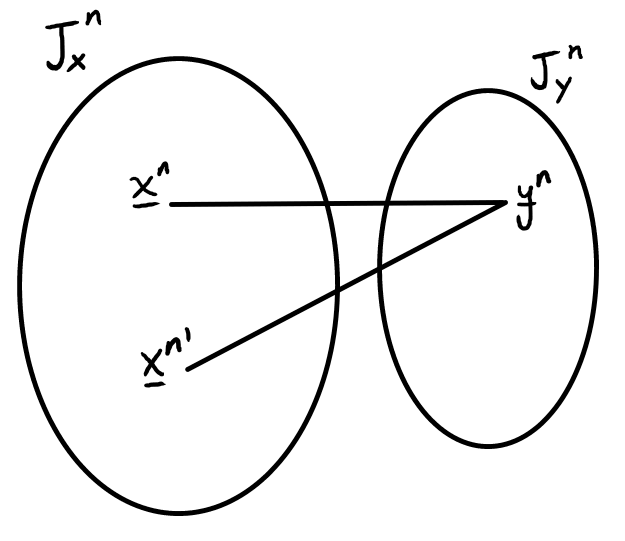
\includegraphics[width=0.35\textwidth]{lent/qi/2019/01/20190125_noisychannel1.png}
    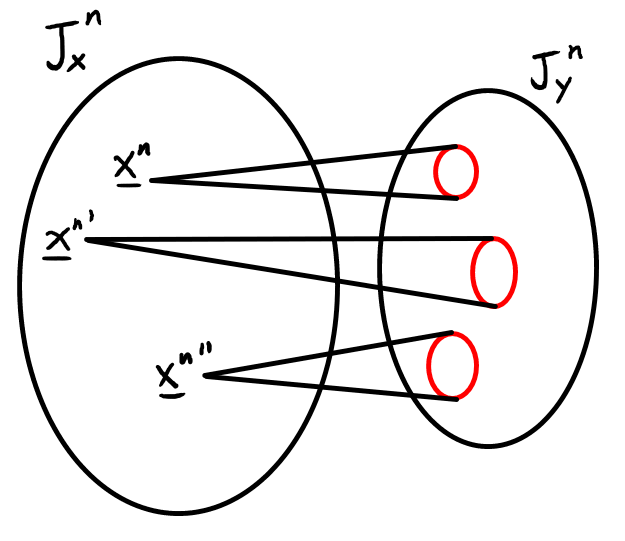
\includegraphics[width=0.35\textwidth]{lent/qi/2019/01/20190125_noisychannel2.png}
    \caption{In a noisy channel, it might be the case that multiple inputs map to the same output, as in the left set of ovals. Both $\underline{x}^n$ and $\underline{x}^n{}'$ have been mapped to the same $\underline{y}^n$ with some probability. However, Shannon tells us that certain codewords will be transmitted as disjoint regions (red ovals) after being sent through the channel, so those codewords can be reliably decoded after transmission.}
    \label{fig:noisychannel}
\end{figure}

We won't do the full proof of the theorem today, but we can introduce the setup. Suppose Alice has a message $[M]=\set{1,2,\ldots, M}$ she would like to send to Bob. She has a noisy channel $\mathcal{N}:J_X \to J_Y$ with some transition probabilities $p(\underline y^{n}| \underline x^{n})$.

%encoding-decoding Tikz figure
\begin{center}
    \begin{tikzpicture}[scale=2, node distance = 2.5cm]
        %make nodes
        \node [] (start) {};
        \node [block, right of=start] (encoding) {$\mathcal{E}_n$};
        \node [block, right of=encoding] (channel) {$\mathcal{N}$};
        \node [block, right of=channel] (decoding) {$\mathcal{D}_n$};
        \node [right of=decoding] (end) {};
        
        %make lines
        \path [line] (start) -- node[below] {$m\in M$} (encoding);
        \path [line] (encoding) -- node[below] {$x_m$} (channel);
        \path [line] (channel) -- node[below] {$y_m$} (decoding);
        \path [line] (decoding) -- node[below] {$m'$} (end);
    \end{tikzpicture}
\end{center}

\begin{enumerate}
    \item First, Alice can choose an encoding scheme $\mathcal{E}_n:[M]\to J_X^n$ where $\forall m\in [M], \mathcal{E}_n(m)=\underline x^{(n)} \in J_X^n$.
    \item She then sends her message through the channel $\mathcal{N}^{(n)}:x^{(n)}\to y^{(n)}$, producing some transmitted messages $y^{(n)}$ with some given probabilities.
    \item Bob receives the message and performs the decoding with $\mathcal{D}_n$ to get some decoded message $\mathcal{D}_n(\mathcal{N}^{(n)}(\mathcal{E}_n(M)))=m'$.
\end{enumerate}

Thus the \term{maximum probability of error} is
\begin{equation}
    \max{m\in [M]} P(\mathcal{D}_n(\mathcal{N}^{(n)}(\mathcal{E}_n(M))) \neq m) = p(\mathcal{E}_n,\mathcal{D}_n).
\end{equation}
We say that the \term{rate} is the number of the bits of the message transmitted per use of the channel. That is,
\begin{equation}
    R= \frac{\log M}{n}
\end{equation}
since $M \approx 2^{\lfloor nR \rfloor}.$

\begin{defn}
    We say that a rate is $R$ is \term{achievable} if there exists a sequence $(\mathcal{E}_n, \mathcal{D}_n)$ with $M=2^{nR}$ such that
    \begin{equation}
        \lim_{n\to \infty} p(\mathcal{E}_n,\mathcal{D}_n)= 0,
    \end{equation}
    i.e. the maximum probability of error tends to zero as $n$ goes to $\infty$.
\end{defn}

We make one final definition for today.
\begin{defn}
    The \term{channel capacity} is defined to be
    \begin{equation}
        C(\mathcal{N})=\sup \set{R: R\text{ is an achievable rate}},
    \end{equation}
    the maximum achievable rate for a channel.
\end{defn}

\subsection*{Non-lectured: m.b.s.c encoding}

For Example \ref{exm:mbsc}, we were asked to consider a binary channel $N$ with error probability $p$. That is, if we give it an input $x\in \set{0,1}$, we get an output $N(x)=y\in \set{0,1}$ such that $p(N(x)\neq x)=p$.

We came up with the following encoding scheme: send $0\mapsto 000$ and $1\mapsto 111$. To decode, we simply take a majority vote, e.g. $010$ was ``probably'' $000$, so the original message was $0$. Now how much better can we do with this redundancy? Let's consider the possible inputs, how they would be encoded, and how often they would be correct.

Suppose we want to send $0\mapsto 000$.
\begin{itemize}
    \item With probability $(1-p)^3$, none of the three bits are flipped and we get $000$ as the output. The process succeeds.
    \item With probability $3\times p(1-p)^2$, exactly one of the three bits is flipped. (The factor of $3$ comes from the fact that we could have flipped any of the three.) We still succeed.
    \item If two or three bits are flipped, we definitely fail.
\end{itemize}
By the symmetry of the problem, the success and failure probabilities are the same for $1\mapsto 111$.

Let's add this up to get the total success probability:
\begin{equation}
    (1-p)^3+3p(1-p)^2=(1+2p)(1-p)^2.
\end{equation}
When $p=1/2$, the success probability of our scheme is
\begin{equation}
    (1+2p)(1-p)^2=(2)(1/2)^2=1/2.
\end{equation}
We can nicely visualize this with the following graphic:
\begin{center}
    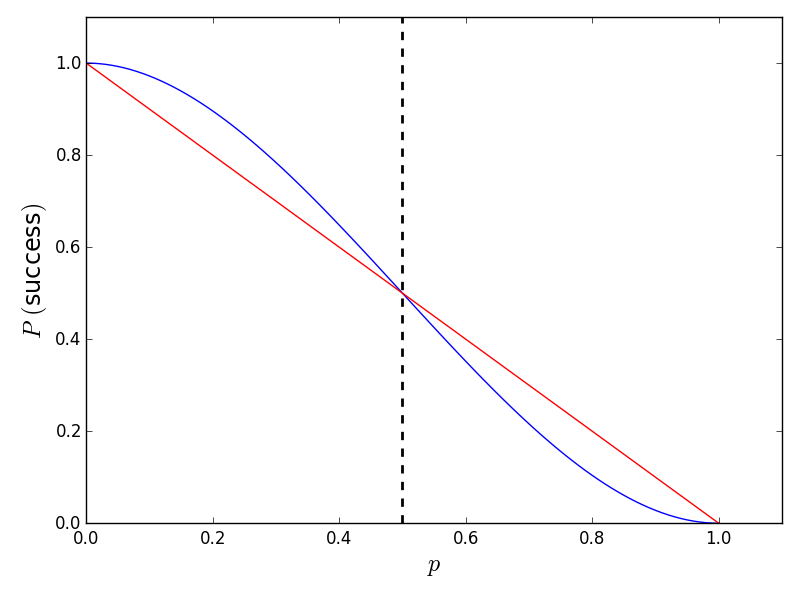
\includegraphics[width=0.5\textwidth]{2019/01/20190125_redundancy.png}
\end{center}
Here, the curved blue line is our three-bit scheme and the red line is the single-bit success probability $1-p$. For completeness, we can explicitly show that the crossover points occur when $P(\text{three bits})-P(\text{one bit})=(1+2p)(1-p)^2-(1-p)=0.$ Rewriting, we have $(1-p)(1-2p)p=0$, which clearly has zeroes at $p=0,1/2,1$. If we now take a derivative, we see that $\frac{d}{dp}\paren{P(\text{three bits})-P(\text{one bit})}|_{p=1/2}=1-6(1/2)+6(1/2)^2=-1/2,$ so $P(\text{three bits})>P(\text{one bit})$ for $p<1/2$.
    
\section{Monday, January 28, 2019}
    Last time, we began discussing the quantization of the string. We said that our approach would be to quantize the unconstrained first and then apply the quantum-ized constraint $T_{ab}=0$ on all physical states in the Hilbert space. We do this by imposing the conditions
\begin{equation}
    L_n \ket{\phi}=0, \quad n>0
\end{equation}
for $\ket{\phi}$ to be physical. Note that $\bar L_n\ket{\phi}=0$ as well-- for most of our theory, we'll get an exact copy of the behavior of the right-handed modes $L_n$ in the left-handed modes $\bar L_n$.

We also observed that our definition of $L_0$ was ambiguous in the quantum theory. In the other operators, we always had products of modes $\alpha_n$ with different harmonics $n$, but for $L_0$ there is an ordering ambiguity. We therefor impose the physical condition that
\begin{equation}
    (L_0-a)\ket{\phi}=0, \quad (\bar L_0 -a)\ket{\phi}=0
\end{equation}
where $a\in \RR$ quantifies this ordering ambiguity. We will see later (cf. BRST invariance) that the theory is consistent only if $D=26,a=1$. From now on we shall assume $a=1$.

It will be useful to define
\begin{equation}
    L_0^\pm = L_0 \pm \bar L_0,
\end{equation}
so that we have
\begin{equation}
    (L_0^+ -2)\ket{\psi}=0,\quad L_0^- \ket{\psi} = 0, \quad L_n \ket{\psi}=\bar L_n \ket{\psi}=0, n>0.
\end{equation}
These three conditions characterize physical states. Recall that $L_0=\frac{\alpha'}{4} p^2 + N, \bar L_0=\frac{\alpha'}{4} p^2 + \bar N$.

\subsection*{The spectrum} We'll start by looking at the lowest-lying modes of the theory. We haven't yet discussed the creation or destruction of strings, so the following discussion will, if you like, be centered on free propagators.

We begin by remarking that in our version of the theory, there are problems in the infrared which have to do with \term{tachyons}. These problems can be addressed in superstring theory, which is beyond the scope of this course.

The simplest state we can write down is the momentum eigenstate,
\begin{equation}
    \ket{k}=e^{ik\cdot x}\ket{0},
\end{equation}
with $k_\mu$ some four-vector of our choice and $x$ the center of mass coordinate for the string (i.e. the $x$ such that $X^\mu(\sigma, \tau)=x^\mu+p^\mu \tau+{}$oscillations).
The action of the center of mass momentum $p_\mu$ is then
\begin{equation}
    p_\mu \ket{k}= k_\mu \ket{k}.
\end{equation}

We could define a general state by a weighted sum of these momentum eigenstates,
\begin{equation}
    \ket{T}=\int d^Dk\, T(k) \ket{k},
\end{equation}
where $T(k)$ is a function of our choosing and we are working in $D$ dimensions. Now the $L_0^-\ket{\phi}=0$ condition imposes $N=\bar N$. This is called the ``level-matching'' condition. It turns out to be the only condition that relates the left-going and right-going modes-- otherwise, they are totally uncoupled.

If we look at $L_0^+$, we get the condition
\begin{equation}
    (L_0^+ -2)T(k)\ket{k}= \paren{ \frac{\alpha'}{2}p^2 + N +\bar N -2} T(k) \ket{k}=0,
\end{equation}
which tells us that $N=\bar N = 0$. Therefore
\begin{equation}
    (L_0^+ -2)T(k)\ket{k}= \paren{ \frac{\alpha'}{2}p^2-2} T(k) \ket{k}=0,
\end{equation}
which we can rewrite as a mass-shell condtion on the momentum space field $T(k)$:
\begin{equation}
    (k^2+M^2) T(k)=0\quad\text{where } M^2=-\frac{4}{\alpha'}.
\end{equation}
We notice that the field $T(k)$ is tachyonic, i.e. its mass squared is negative. (We use the mostly $+$ sign convention for the Minkowski metric.) Note that
\begin{equation}
    L_n\ket{T}=0 =\bar L_n\ket{T} \text{ for }n>0
\end{equation}
is satisfied trivially. A priori, tachyons need not sink our theory. It could be that we're just working relative to the wrong vacuum. This is an open question, though there are other reasons the bosonic string might not be quite the right model for our universe's physics. Having declared that superstring theory does provide some solution to this problem, we will pay it no more thought and move on.

\subsection*{Massless states}
Next, we consider states of the form
\begin{equation}
    \ket{\epsilon}=\epsilon_{\mu\nu}(k) \alpha_{-1}^\mu \bar \alpha_{-1}^\nu \ket{k},
\end{equation}
where we have included both $\alpha$ and $\bar \alpha$ to satisfy level-matching, and we have thrown in an $\epsilon$ in order to kill the free indices.

The condition $(L_0^+-2) \ket{\epsilon}=0$ gives $M^2=0$ since $N=\bar N = 1$. Note that $L_n \ket{\epsilon}=0$ is satisfied trivially for $n>1$ (and so is $\bar L_n \ket{\epsilon}=0$).

What about $L_1\ket{\epsilon}=0$? We have
\begin{align*}
    L_a \ket{\epsilon} &= \frac{1}{2} \sum_n \alpha_{1-n} \cdot \alpha_n \epsilon_{\mu\nu} \alpha_{-1}^\mu \bar \alpha_{-1}^\nu \ket{k}\\
    &= \epsilon_{\mu\nu}(k) \alpha_0 \cdot \alpha_1 \alpha_{-1}^\mu \bar \alpha_{-1}^\nu \ket{k}\\
    &=\sqrt{\frac{2}{\alpha'}} \epsilon_{\mu\nu} (k) k_\lambda \a_1^\lambda \a_{-1}^\mu \bar \a_{-1}^\nu \ket{k}\\
    &=\sqrt{\frac{2}{\a'}} \epsilon_{\mu\nu} (k) k_\lambda \paren{[\a_1^\lambda, \a_{-1}^\lambda]+\a_{-1}^\mu \a_1^\lambda} \bar \a_{-1}^\nu\ket{k}.
\end{align*}
We conclude that
\begin{equation}
    \epsilon_{\mu\nu}(k)k^\mu =0,
\end{equation}
so two states related by
\begin{equation}
    \epsilon_{\mu\nu}(k)\to \epsilon_{\mu\nu}(k) + k_\mu \xi_\nu
\end{equation}
are physically equivalent since $k^2=0$, with $\xi$ arbitrary. Similarly,
\begin{equation}
    \bar L_1\ket{\epsilon}=0 \implies k^\nu \epsilon_{\mu\nu}(k)=0.
\end{equation}
It is useful to decompose $\epsilon_{\mu\nu}(k)$ as follows:
\begin{equation}
    \epsilon_{\mu\nu}(k)=\tilde g_{\mu\nu}(k) + \tilde B_{\mu\nu}(k)+\eta_{\mu\nu} \tilde \phi(k),
\end{equation}
where $\tilde g_{\mu\nu}$ is traceless symmetric and $\tilde B_{\mu\nu}$ is antisymmetric. Now $\tilde g_{\mu\nu}(k)$ has the interpretation of a momentum space metric perturbation,
\begin{equation}
    \tilde g_{\mu\nu}(k) \sim \tilde g_{\mu\nu}(k) + k_\mu \xi_\nu + \xi_\mu k_\nu,
\end{equation}
which is simply (linearized) diffeomorphism invariance. What about this antisymmetric guy? We get a ``$B$-field'' which corresponds to a momentum spacetime field $\tilde B_{\mu\nu}=-\tilde B_{\nu\mu}$, where
\begin{equation}
    \tilde B_{\mu\nu} (k) \sim \tilde B_{\mu\nu}(k)+k_\mu \lambda_\nu - k_\nu \lambda_\mu.
\end{equation}
In spacetime this is a gauge invariance, where $B_{\mu\nu}\sim B_{\mu\nu} + \p_\mu \lambda_\nu - \p_\nu \lambda_\mu.$ Some older textbooks call this the notoph (which is nearly ``photon'' backwards).
    
\section{Wednesday, January 30, 2019}
    Today, we shall begin our discussion of quantum information theory. First, a quick review of Dirac's bra-ket notation-- we denote a vector in Hilbert space $\cH =\CC^d$ by
\begin{equation}
    \ket{v} = \begin{pmatrix}
    v_1\\ \vdots \\ v_d
    \end{pmatrix},
\end{equation}
and call this a \term{ket}. We also have the dual vectors (row vectors, if you like), called \term{bras}. such that
\begin{equation}
    \bra{v}=(v_1^*, \ldots, v_d^*).
\end{equation}
The braket notation provides us with a natural inner product:
\begin{equation}
    (u,v)=\braket{u}{v}=\sum_{i=1}^d u_i^* v_i.
\end{equation}
This space also comes equipped with an outer product, $\ket{u}\bra{v}$, which is the matrix
\begin{equation}
    \ket{u}\bra{v} =\begin{pmatrix}
    u_1 v_1^* &\ldots&\\
    \vdots\\
    u_d v_1^* &\ldots &u_d v_d^*
    \end{pmatrix}.
\end{equation}
We can then take an orthonormal basis (onb) for $\cH$, which we denote by $\set{\ket{e_i}}$ with $\braket{e_i}{e_j}=\delta_{ij}$. Note that for any basis of $\cH$, we can write the identity matrix as
\begin{equation}
    I=\sum_{i=1}^d \ket{e_i}\bra{e_i}.
\end{equation}
There is a nice basis $\ket{e_1}=\begin{pmatrix}1\\0\\\vdots\\0\end{pmatrix}$ we can write down,
so that for a general basis $\set{\ket{f_i}}_{i=1}^d$ related to the original by a unitary $U$, we find that
\begin{equation}
    \sum_{i=1}^d \ket{f_i}\bra{f_i}=\sum_{i=1}^d U \ket{e_i} \bra{e_i} U^\dagger = U I U^\dagger =UU^\dagger = I.
\end{equation}

Now in classical information, our simplest system was a binary bit, a system taking values $0$ and $1$. For quantum information theory, we have a \term{qubit}, a two-level system represented by a Hilbert space with $\cH=\CC^2$ and basis vectors $\set{\ket{0},\ket{1}}$ or equivalently $\set{\ket{\uparrow},\ket{\downarrow}}.$ Physically, these could be the spin states of an electron or perhaps the polarizations of a photon.

Now, it is obvious that any state in Hilbert space can be decomposed in the basis of our choice, i.e.
\begin{equation}
    \ket{\psi}=a\ket{0}+b\ket{1},
\end{equation}
with $a,b\in \CC$. We shall require that our states are normalized under this inner product, so that
\begin{equation}
    1=\braket{\psi}{\psi}=|a|^2+|b|^2,
\end{equation}
which means that $|a|^2$ and $|b|^2$ have the interpretation of probabilities.

We also have some important operators on Hilbert space. These are the Pauli matrices%fill in the pauli matrices
$\sigma_0,\sigma_x,\sigma_y,\sigma_z$. As it turns out, these operators form a basis. Note that we have a set of self-adjoint $2\times 2$ complex matrices
\begin{equation}
    B_{SA}(\CC^2)=\set{A\in B(\cH): A=A^\dagger},
\end{equation}
and we can write a general matrix $M\in M_2 /M_{sa}$ in terms of the Pauli matrices,
\begin{equation}
    M=\frac{1}{2}(x_0 \sigma_0 +\vec x \cdot \gv \sigma),
\end{equation}
where $\vec x=(x_1,x_2,x_3)\in \RR^3$.

\subsection*{Spectral decomposition}
The spectral decomposition says that we can write a matrix in terms of its eigenvalues,
\begin{equation}
    A=\sum_{i=1}^d \lambda_i \ket{e_I}\bra{e_i},
\end{equation}
such that $A\ket{e_i}=\lambda_i \ket{e_i}$. Sometimes, we say that the eigenvalue decomposition is written in terms of projectors instead,
\begin{equation}
    A=\sum_{i=1}^m \lambda_i \Pi_i
\end{equation}
where $\Pi_i$ projects onto some basis.

Given a self-adjoint operator $A=A^\dagger$ and a nice function $f$, what is the value $f(A)$? Note that $A$, being self-adjoint, can be diagonalized by a unitary. Thus
\begin{equation}
    A_d = UAU^\dagger \implies A = U^\dagger A_d U,
\end{equation}
so that
\begin{equation}
    f(A)=U^\dagger \begin{pmatrix}
    f(\lambda_1) && \\
    & \ddots & \\
    && f(\lambda_d)
    \end{pmatrix}.
\end{equation}
Thus for example
\begin{equation*}
    f(A)=e^{iA}=I + iA +\frac{i^2}{2!}+\ldots.
\end{equation*}

\subsection*{QM postulates}
We consider the following postulates of quantum mechanics, which will in fact be qualified by the fact we are working in an open system.
\begin{enumerate}
    \item The state of a (closed) system is given by a ray in $\cH$, i.e. a vector defined up to a global phase. Thus we cannot distinguish a state $\ket{\psi}$ and $e^{i\phi}\ket{\psi}$ by any physical measurement. We traditionally take a representative of this equivalence class, $\ket{\psi}.$
\end{enumerate}
For an open system $A$, consider a system which is in states $\ket{\psi_i}$ with some coefficients $p_i, i=1,\ldots, m$. The state is characterized by an ensemble
\begin{equation}
    \set{p_i,\ket{\psi_i}}_{i=1}^m.
\end{equation}
Note that these $\ket{\psi_i}$s need not be mutually orthogonal,
\begin{equation}
    \braket{\psi_i}{\psi_j}\neq \delta_{ij},
\end{equation}
and moreover this is \emph{not} a superposition but a statistical mixture. A superposition is a pure state where the state is normalized and can be written as 
\begin{equation}
    \ket{\Psi}=\sum_{i=1}^d a_i \ket{\phi_i}.
\end{equation}

So a statistical mixture is instead described by a \term{density matrix} (or density operator). We could write our ensemble as
\begin{equation}
    \rho \equiv \sum_{i=1}^m p_i \ket{\psi_i} \bra{\psi_i},
\end{equation}
noting that the $\ket{\psi_i}$s in general \emph{need not be orthogonal}.
\begin{defn}
    A \term{density matrix} on $\cH$ ($\dim \cH = d$) is an operator $\rho$ with the following properties:
    \begin{itemize}
        \item $\rho \geq 0$, i.e. $\rho$ is positive semi-definite, $\bra{\phi}\rho \ket{\phi}\geq 0,$ which implies that $\rho=\rho^\dagger$.
        \item $\Tr \rho =1$ (which gives it a probabilistic interpretation).
    \end{itemize}
\end{defn}
Let us remark that $\rho$ is hermitian and therefore admits a spectral decomposition, i.e.
\begin{equation}
    \rho = \sum_{j=1}^d \lambda_j \ket{e_j}\bra{e_j}
\end{equation}
in terms of an orthonormal basis. Thus
\begin{equation}
    \rho=\sum_{i=1}^m p_i \ket{\psi_i}\bra{\psi_i} = \sum_{j=1}^d \lambda_j \ket{e_j} \bra{e_j}.
\end{equation}
We will prove on Examples Sheet 2 that the set
$\mathcal{D}(\cH)$ of density matrices is a complex set.

\subsection*{Pure and mixed states} 
Consider a density matrix
\begin{equation}
    \rho = \sum p_i \ket{\psi_i}\bra{\psi_i},
\end{equation}
and suppose for example that $p_2=1, p_i=0 \forall i\neq 2$. Then
\begin{equation}
    \rho=\ket{\psi_2}\bra{\psi_2}.
\end{equation}
This is very nice, because we know precisely the state of the system (or equivalently the outcome of applying the operator $\rho$). We call this a \term{pure state}, referring either to the vector $\ket{\psi_2}$ or the operator $\ket{\psi_2}\bra{\psi_2}$. Otherwise, $\rho$ is a \term{mixed state}.

A pure state will have $\rho^2 = \rho$, so we can define the \term{purity} of a state by $\Tr \rho^2$. Conversely, we can define a completely mixed state by
\begin{equation}
    \rho = I/d=\frac{1}{d} \sum_{i=1}^d \ket{e_i} \bra{e_i},
\end{equation}
such that a completely mixed state has purity $1/d$ (where we get a factor of $d$ from taking the trace of $I$).

In classical probability, we remark that the convex set of probability distributions forms a \term{simplex}.

Now let's briefly discuss the expectation value of an observable (self-adjoint operator) in $B(\cH)$. For a state $\rho$, we define the expectation value to be
\begin{equation}
    \phi(A) \equiv \avg{A}_\rho =\Tr(A \rho).
\end{equation}
This is a linear normalized functional--
\begin{itemize}
    \item $\phi(aA +b B) = a\phi(A) + b\phi(B)$
    \item $\phi(A)\geq 0$ with equality when $A=I$.
\end{itemize}

\section{Thursday, January 31, 2019}
    Today we'll finish our discussion of the zero-dimensional path integral by introducing fermions to our theory. To model fermions, we will introduce Grassmann variables,%
    \footnote{We've seen these in \emph{Supersymmetry} already.
    }
i.e. a set of $n$ elements $\set{\theta_a}_{a=1}^n$ obeying anticommutation relations,
\begin{equation}
    \theta_a \theta_b = -\theta_b \theta_a.
\end{equation}
Note also that for (complex) scalars $\phi_b\in \CC$,
\begin{equation}
    \theta_a \phi_b = \phi_b \theta_a,
\end{equation}
i.e. scalars commute with Grassmann variables. In addition, $\theta^2_a =0$ by the anticommutation relations, which implies that any function of $n$ Grassmann variables can be written in finite form. That is, polynomials in Grassmann variables are forced to terminate since at some point we run out of distinct Grassmann variables to multiply. A general function $F(\theta)$ can be written
\begin{equation}
    F(\theta)=f+\rho_a \theta_a +\frac{1}{2!} g_{ab} \theta_a \theta_b + \ldots + \frac{1}{n!} h_{a_1\ldots a_n} \theta_{a_1}\ldots \theta_{a_n}.
\end{equation}
Note that the coefficients $\rho,g,\ldots,h$ are totally antisymmetric under interchange of indices.

We also want to define differentiation and integration of these guys. Differentiation anticommutes with the Grassmann variables, i.e.
\begin{equation}
    \paren{\P{}{\theta_a}\theta_b + \theta_b \P{}{\theta_a}} * = (\delta_{ab})*
\end{equation}
where the derivative in the first term acts on everything coming after. This leads us to a modified Leibniz rule.

To define integration, note that for a single Grassmann variable $\theta$, a function takes the form
\begin{equation}
    F(\theta)=f+\rho \theta,
\end{equation}
so we just need to define $\int d\theta$ and $\int d\theta \,\theta$. If we require translational invariance, i.e.
\begin{equation}
    \int d\theta(\theta+\eta)=\int d\theta \theta \implies \int d\theta =0.
\end{equation}
We can then choose the normalization so that $\int d\theta \, \theta = 1$. Note the similarity between differentiation and integration (i.e. an integral $\int d\theta\,\theta =\P{}{\theta}\theta=1$). This process is called \term{Berezin integration}. Using these rules, we also find that
\begin{equation}
    \int d\theta \P{}{\theta} F(\theta)=0,
\end{equation}
since the term linear in $\theta$ will go to a constant by the derivative and be killed by the integral, and any constant terms will be killed by the derivative. Either way the result is zero.

Suppose now we have $n$ Grassmann variables. Then the only nonvanishing integrals involve exactly one power of each integration variable, e.g.
\begin{equation}
    \int d^n \theta\, \theta_1 \theta_2 \ldots \theta_n = \int d\theta_n d\theta_{n-1}\ldots d\theta_1 \, \theta_1 \theta_2 \ldots \theta_n = 1.
\end{equation}
In general we can just anticommute the Grassmann variables until they're in the right order, picking up a factor for the parity of the permutation. That is,
\begin{equation}
    \int d^n\theta \theta_{a_1}\theta_{a_2}\ldots \theta_{a_n} = \epsilon^{a_1 a_2 \ldots a_n},
\end{equation}
where $\epsilon$ is the totally antisymmetric symbol with value $+1$ for even permutations of $1,2,\ldots,n$, $-1$ for odd permutations, and $0$ if any indices are repeated.

What if we now make a change of variables $\theta_a' = A_{ab} \theta_b$? Then
\begin{align}
    \int d^n \theta \theta'_{a_1} \theta'_{a_2} \ldots \theta'_{a_n} &= A_{a_1b_1}\ldots A_{a_nb_n} \underbrace{\int d^n \theta \, \theta_{b_1} \ldots \theta_{b_n}}_{\epsilon^{b_1\ldots b_n}}\\
    &= \det A \,\epsilon^{a_1\ldots a_n}\\
    &= \det A \int d^n \theta' \,\theta'_{a_1} \ldots \theta'_{a_n}
\end{align}
We conclude that under a change of variables, the integration measures are related by
\begin{equation}
    d^n\theta = \det A \,d^n \theta'.
\end{equation}
Note that this is the opposite of the convention for scalars, where
\begin{equation}
    \phi'_a = A_{ab} \phi_b \implies d^n \phi =\frac{1}{|\det A|}d^n \phi'.
\end{equation}

\subsection*{Free fermion field theory} Consider $d=0$, with two fermion fields $\theta_1,\theta_2$. The action must be bosonic (scalar), so the only possible nonconstant action is
\begin{equation}
    S(\theta)=\frac{1}{2}A \theta_1 \theta_2, A\in \RR
\end{equation}
Then the path integral is
\begin{equation}
    Z_0 = \int d^2 \theta \, e^{-S(\theta)/\hbar}=\int d^2\theta \paren{ 1-\frac{A}{2\hbar}\theta_1\theta_2} = -\frac{A}{2\hbar},
\end{equation}
where the exponential has terminated thanks to our Grassmann variables.

Suppose now we have $n=2m$ fermion fields $\theta_a$. Then our action might be quadratic in the fields,
\begin{equation}
    S=\frac{1}{2} A_{ab} \theta_a \theta_b
\end{equation}
with $A$ an antisymmetric matrix, and the path integral is then
\begin{align*}
    Z_0 &= \int d^{2m}\theta\, e^{-S(\theta)/\hbar} = \int d^{2m} \theta \sum_{j=0}^{m} \frac{(-1)^j}{(2\hbar)^j j!} (A_{ab}\theta_a \theta_b)^j\\
    &= \frac{(-1)^m}{(2\hbar)^m m!} \int d^{2m}\theta A_{a_1 a_2} A_{a_3 a_4} \ldots A_{a_{2m-1} a_{2m}} \theta_{a_1} \theta_{a_2} \ldots \theta_{2m}\\
    &= \frac{(-1)^m}{(2\hbar)^m m!} \epsilon^{a_1 a_2 \ldots a_{2m}} A_{a_1 a_2} A_{a_3 a_4} \ldots A_{a_{2m-1} a_{2m}}\\
    &= \frac{(-1)^m}{\hbar^m} \text{Pf}(A),
\end{align*}
where $\text{Pf}(A)$ is the \term{Pfaffian} of the matrix $A$, defined by
\begin{equation}
    \text{Pf}(A)\equiv \frac{1}{2^m} \epsilon^{a_1 a_2 \ldots a_{2m}} A_{a_1 a_2} A_{a_3 a_4} \ldots A_{a_{2m-1} a_{2m}},
\end{equation}
which we will show on the examples sheet is in fact $\pm \sqrt{\det A}.$ Thus $\text{Pf}\begin{pmatrix}0 & -1 \\ a & 0 \end{pmatrix} = a$. Using this property, we find that for fermionic fields,
\begin{equation}
    Z_0 = \pm \sqrt{\frac{\det A}{\hbar^n}}
\end{equation}
with $A$ antisymmetric, whereas for bosonic fields with some symmetric mass matrix $M$,%
    \footnote{That is, for an action $S=\frac{1}{2}M_{ab}\phi_a \phi_b$.}
we have
\begin{equation}
    Z_0=\sqrt{\frac{(2\pi \hbar)^n}{\det M}}.
\end{equation}

We can now introduce an external source function to our action, a Grassmann-values $\set{\eta_a}$, such that the new action is
\begin{equation}
    S(\theta,\eta)=\frac{1}{2} A_{ab} \theta_a \theta_b + \eta_a \theta_b.
\end{equation}
Taking care to respect the anticommutation relations and completing the square as before, we can rewrite the action as
\begin{equation}
    S(\theta,\eta)=\frac{1}{2}(\theta_a +\eta_c(A^{-1})_{ca}) A_{ab}(\theta_b +\theta_d(A^{-1})_{db}) +\frac{1}{2} \eta_a (A^{-1})_{ab} \eta_b.
\end{equation}
We can make a change of variables using the translational invariance of $\theta_a$ and pull out the constant factor to find
\begin{equation}
    Z_0(\eta)=\exp\paren{-\frac{1}{2\hbar}\eta^T( A^{-1}) \eta} Z_0(0).
\end{equation}
This allows us to get propagators by taking derivatives with respect to the source $\eta$, as we are wont to do:
\begin{equation}
    \avg{\theta_a \theta_b}
    = \frac{\hbar^2}{Z_0(0)}\frac{\p^2 Z_0(\eta)}{\p \eta_a \p \eta_b}|_{\eta=0} 
    = \hbar(A^{-1})_{ab}.
\end{equation}
We see that the propagator is proportional to the inverse of the bilinear part of the action for Grassmann variables.

\section{Friday, February 1, 2019}
    Let us now continue our discussion of path integral quantization. Heuristically, we'll \begin{verbatim}import\end{verbatim} the details of path integral quantization and see what works out. We want to understand how to make sense of expressions like
\begin{equation}
    \int \cD h \cD X \,e^{iS[h,X]}
\end{equation}
where we are integrating over the space of metrics $h_{ab}$ and embedding fields $X^\mu$s. When we do this calculation, we have to be careful not to overcount-- there is a huge diffeomorphism symmetry and a Weyl symmetry in our theory relating physically equivalent states. If this path integral is to give us anything physically meaningful, we need to ``quotient out'' by the space of diffeomorphisms and Weyl transformations.

We would like to split the integral over all $h_{ab}$ into integrals over physically inequivalent $h_{ab}$ and those related by gauge transformations. Schematically,
\begin{equation}
    \cD h = \cD h_{\text{phys}}\times \mathcal{J}\cD h_{\text{Diff}\times \text{Weyl}},
\end{equation}
where $\mathcal{J}$ is a Jacobian factor whose importance we'll see in the following example.

\begin{exm}
    As a toy example, consider the following integral:
    \begin{equation*}
        \int dxdy\, e^{-(x^2 +y^2)}.
    \end{equation*}
    But notice that $x^2+y^2$ is invariant under rotations about the origin. When we pass to polar coordinates, the $\theta$ angular integral becomes totally trivial, so we might really be interested in this integral modulo rotations. Thus our integral can be rewritten
    \begin{equation*}
        \int d\theta \int dr \, re^{-r^2}.
    \end{equation*}
    This $\int d\theta$ will always give us a factor of $2\pi$ (the  ``volume'' of an orbit of the rotation group)-- the real interest is in the $dr$ integral.
\end{exm}

In this example, we needed the Jacobian of the coordinate transformation: $dxdy=rdr d\theta$. The same is true of our path integral. Formally, we will take
\begin{equation}
    \frac{1}{|\text{Diff}|\times |\text{Weyl}|}\int \cD h \cD X = \int \cD h_{\text{phys}}\cD S_{\text{phys}} \,\mathcal{J},
\end{equation}
where $\mathcal{J}$ is now a functional determinant and $|\text{Diff}|, |\text{Weyl}|$ represents the orbits of diffeomorphisms and Weyl transformations.
%
In the same way we could write
\begin{equation}
    \sqrt{\frac{\pi}{\det M}}=\int_V dx \,e^{-(x,Mx)},
\end{equation}
we will write $\mathcal{J}$ as a functional integral,
\begin{equation}
    \cJ =\int \cD b \cD c\, e^{-S[b,c]}.
\end{equation}

\subsection*{Global properties of the worldsheet} We need to know more about what type of worldsheets appear in the path integral. This will take us on a crash course through Riemann surfaces.

We have looked at 2-dimensional Riemannian manifolds $(\Sigma,h)$ modulo Weyl transformations. The set of Riemannian manifolds modulo Weyl transformations is known as \term{Riemann surfaces}. Quotienting out by diffeomorphisms is assumed. Note that worldsheets are Riemann surfaces.

We'll state a number of results without proof, though some of them are not too hard to prove-- for more detail, see Farkas and Kra, and also Donaldson.

The first idea we'll consider is the \term{worldsheet genus}. For Riemann surfaces without boundary (i.e. a closed string, neglecting the initial and final string states), the relevant topological data is encoded in the \term{Euler characteristic},
\begin{equation}
    \chi = \frac{1}{4\pi} \int_\Sigma d^2 \sigma \,\sqrt{h} R(h).
\end{equation}
Here, $R(h)$ is the Ricci scalar with respect to the worldsheet metric $h$. The Euler characteristic captures the idea that while we can locally make the metric look however we want, in general there will be obstructions to globally bringing the metric to a required form. The \term{genus} $g$ is given by
\begin{equation}
    \chi = 2-2g,
\end{equation}
and informally counts the ``number of holes in $\Sigma$.'' Why we care is because the genus is a topological invariant. We can't change the number of holes in a Riemann surface under smooth maps.

\subsection*{Moduli space of Riemann surfaces} For a given genus $g$, the space of metrics on $\Sigma_g$ modulo Weyl and diffeomorphisms is a finite-dimensional space called the \term{moduli space}. Schematically,
\begin{equation*}
    \cM_g = \frac{\set{\text{metrics }h_{ab}}}{\set{\text{Diff}}\times \set{\text{Weyl}}}.
\end{equation*}
Both the numerator and denominator here are infinite dimensional, but our saving grace will be the following fact-- the integral itself is finite-dimensional.

A useful result is the following: let $s$ be the real dimension of the moduli space $\cM_g$. Then
\begin{equation}
    s=\dim \cM_g =\begin{cases}
    0, & g=0\\
    2, & g=1\\
    6g-6, & g\geq 2.
    \end{cases}
\end{equation}

\begin{exm}
    Given a metric $\hat h_{ab}$ on a $g=0$ surface, we can bring any metric to the form $e^{2w}\hat h_{ab}$. This is not the case for a torus ($g=1$). We can build a torus by imposing identifications on $\CC,$ i.e. under the equivalence relation
    \begin{equation}
        z\sim z + n \lambda_1 + m\lambda_2,
    \end{equation}
    where $n,m\in \ZZ$ and $\lambda_1,\lambda_2$ specify the ``dimensions'' of the torus.
    
    One can show that the ratio $\tau\equiv \lambda_1/\lambda_2$ is Diff and Weyl invariant. However, we can always choose $\lambda_1,\lambda_2$ such that $\Im (\tau)\geq 0$. We also get a metric
    \begin{equation}
        ds^2=\abs{dz+\tau d\bar z}^2.
    \end{equation}
    If we transform $\begin{pmatrix}\lambda_1 \\lambda_2\end{pmatrix}\to U\begin{pmatrix}\lambda_1 \\lambda_2\end{pmatrix}$ for some matrix $U$, then we can undo that change by also changing the equivalence relation numbers $(n,m)\to (n,m)U^{-1}$. For $n,m$ to be integers under any such transformation, we require the entries of $U$ to all be integers, i.e. $U\in SL(2,\ZZ)$.
    
    Our moduli space is
    \begin{equation}
        \cM_1 = \frac{UHP}{SL(2,\ZZ)},
    \end{equation}
    with $UHP$ the upper half-plane, $\tau,\Im \tau \geq 0$.
\end{exm}

\section{Monday, February 18, 2019}
    \begin{quote}
    \textit{``We'll see that the shear in AdS tells us amazing things. Well, we won't see the AdS. But we'll see the amazing thing.'' --Jorge Santos}
\end{quote}
It's been 15 days since the last lecture. Where did we leave off? We introduced null surfaces, and suggested that null surfaces will be important to our understanding of singularity theorems.
%Today will be the second hardest class of the whole course.

Last time, we talked about geodesic congruences (families of geodesics which cover some submanifold of the spacetime). Consider a congruence where all geodesics are of the same type,
\begin{equation*}
    U^a U_a = \pm 1
\end{equation*}
in affine parametrization (for spacelike or timelike geodesics respsectively) or $U^a U_a =0$ for null congruences.
Now consider a 1-parameter family of geodesics which form such a congruence. In terms of the geodesic tangent vector $U$ and the deviation vector $S$, we have
\begin{equation}
    [S,U]=0\iff U^b \nabla_b S^a = S^b \nabla_b U^a = S^b B^a{}_b
\end{equation}
where we have defined
\begin{equation}
    B^a{}_b \equiv \nabla_b U^a.
\end{equation}
That is, $B$ measures the failure of $S^a$ to be parallel propagated along $U^b$. This tensor has some nice properties:
\begin{equation}
    B^a{}_b U^b =0, \quad U_a B^a{}_b = \frac{1}{2} \nabla_b(U^2)=0.
\end{equation}
The first follows from the geodesic equation and the latter from $U^2={}$constant.%
    \footnote{Just one line of algebra. $U_a B^a{}_b=U_a \nabla_b U^a = \frac{1}{2} \nabla_b(U^2)=0$.}
Consider the following expression:
\begin{equation}
     U\cdot \nabla(U\cdot S) = (U\cdot \nabla U^a) S_a + U^a (U\cdot \nabla S_a),
\end{equation}
where $(\cdot)$ indicates contracted indices. But this first term is zero by the geodesic equation, and the second is zero by the property $U^a B_{ab}=0$ from above. Thus $U\cdot S$ is constant along the integral curves of $U$.

The existence of some quantity along geodesics suggests to us there might be some gauge freedom we get to fix. In particular, we can make a very nice choice to fix the affine parameter along geodesics:
\begin{equation}
    \lambda'=\lambda - a(s)
\end{equation}
where $a$ is some function of our choice. In particular this allows us to shift $S$:%
    \footnote{Recall that $S\equiv \frac{dx^\mu}{ds}$, and $U^\mu\equiv\frac{dx^\mu}{d\lambda}$. Thus for a geodesic parametrized by $\lambda',s$, we may write
    \begin{align*}
        x^\mu(\lambda',s) &= x^\mu(\lambda-a(s),s)\\
            &= x^\mu(\lambda,s)+\frac{dx^\mu}{d\lambda}a(s)\\
            &= x^\mu(\lambda,s)+U^\mu a(s),\\
    \end{align*}
    and taking a derivative with respect to $s$ now yields
    \begin{equation*}
        \frac{dx^\mu(\lambda',s)}{ds} = \frac{dx^\mu(\lambda,s)}{ds}+\frac{da}{ds}U^\mu.
    \end{equation*}
    }
\begin{equation}
    S'{}^a\equiv S^a +\frac{da}{ds} U^a \implies U\cdot S'=U\cdot S +\frac{da}{ds}U^2.
\end{equation}
What's nice about this? $U^2=\pm 1$ for timelike or spacelike coordinates, which means that WLOG we can set $U\cdot S'=0$. But for the null case, $U^2=0$ means that the reparametrization cannot be fixed by a choice of $a$-- we just get $U\cdot S'=U\cdot S$.

\subsection*{Gauge fixing, the easy way}
For null geodesic congruences, we have $U^2=0$ and thus
\begin{equation*}
    U\cdot S'= U\cdot S,
\end{equation*}
so $a$ doesn't help us pick a nice reparametrization. Instead, we pick a spacelike hypersurface $\Sigma$ which intersects each geodesic once-- we can do this since we're looking at a congruence. Now let $N^a$ be a vector field defined on $\Sigma$ obeying $N^2=0, N\cdot U=-1$ on $\Sigma$.

Now extend $N^a$ off $\Sigma$ by parallel transport along the geodesic
\begin{equation}
    U\cdot \nabla N^a=0.
\end{equation}
There's a nice discussion of equivalence classes and the full freedom we have to fix the gauge, but we'll leave it to Wald. For our purposes, notice that we have the three properties
\begin{equation}
    N^2 = 0, \quad U\cdot N=-1,\quad U\cdot \nabla N^a=0.
\end{equation}
Take a deviation vector $S^a$ and decompose it as follows:
\begin{equation}
    S^a= \alpha U^a +\beta N^a + \hat S^a,
\end{equation}
where
\begin{equation}
    U\cdot \hat S = N\cdot \hat S=0.
\end{equation}
This is a bit like a Gram-Schmidt process-- we can subtract off the bits parallel to the geodesic $U^a$ and also the bit parallel to $N^a$.
Note that $U\cdot S=-\beta$, where $\beta$ is constant, as we found at the start of the calculation. It's also important to observe that any vector which is orthogonal to two null vectors is either spacelike or the zero vector.%
    \footnote{To see this, try the calculation in Minkowski space. I haven't worked out the details myself yet.}

So we can write a deviation vector $S^a$ as the sum of a part
\begin{equation*}
    \alpha U^a + \hat S^a
\end{equation*}
which is orthogonal to $U^a$ and a part
\begin{equation*}
    \beta N^a
\end{equation*}
that is parallel transported along each geodesic.
We are interested in a congruence containing the generators of a null hypersurface $\mathcal{N}$. In this case, if we pick a 1-parameter family of geodesics contained in $\mathcal{N},$ then the deviation vector $S^a$ will be tangent to $\mathcal{N}$ and hence $U\cdot S=0$. Since $U^a$ is normal to $\mathcal{N},$ we have $\beta=0.$

We can write
\begin{equation}
    \hat S^a = P^a{}_b S^b
\end{equation}
under the projection
\begin{equation}
    P^a{}_b = \delta^a{}_b + N^a U_b + U^a N_b,
\end{equation}
where it's a quick exercise to check that $P^a{}_b P^b{}_e = P^a{}_e.$ This projection projects the tangent space at $p$ onto the spacelike $T_\perp$, the space perpendicular to both null vectors $N^a$ and $U^a$.
One can also check that
\begin{equation}
    U\cdot \nabla P^a{}_b =0,
\end{equation}
so $P$ is parallel-propagated trivially along geodesics $U^a$.

\begin{prop}
    A deviation vector for which $U\cdot S=0$ satisfies
    \begin{equation}
        U\cdot \nabla \hat S^a = \hat B^a{}_b \hat S^b,
    \end{equation}
    where $\hat B^a{}_b$ is a projected version of $B^a{}_b$ into the perpendicular space,
    \begin{equation}
        \hat B^a{}_b=P^a{}_c B^c{}_d P_b{}^d.
    \end{equation}
\end{prop}
\begin{proof}
    \begin{align*}
        U\cdot \nabla \hat S^a &= U\cdot \nabla(P^a{}_c S^c)\\
            &= P^a{}c U\cdot \nabla S^c\\
            &= P^a{}_c B^c{}_d S^d\\
            &= P^a{}_c B^c_d P^d{}_e S^e,
    \end{align*}
    where we used $U\cdot S=0$ and $B^c{}_d U^d=0$. Finally, we can use the fact that $P$ is a projector so that $P^2=P$. So we replace $P^d{}_e=P^d{}_f P^f{}_e$ and this gives us the projectors to write everything with hats as
    \begin{equation*}
        U\cdot \nabla \hat S^a = P^a{}_c B^c{}_d P^d{}_f P^f{}_e S^e = \hat B^a{}_f \hat S^f. \qedhere
    \end{equation*}
\end{proof}

\subsection*{Expansion, rotation, and shear}
We've proved some nice properties about this $B^a{}_b$ matrix. But what exactly is it? As it turns out, $\hat B^a{}_b$ can be regarded as a matrix that acts on the $2$D space $T_\perp$. It's very natural for us to decompose such a matrix into its symmetric (trace-free) part, its antisymmetric part, and its trace part.
\begin{defn}
    Let us define
    \begin{equation}
        \theta \equiv \hat B^a{}_a, \quad \hat \sigma_{ab} \equiv \hat B_{(ab)}-\frac{1}{2} P_{ab} \theta, \quad \hat \omega_{ab} = \hat B_{[ab]}.
    \end{equation}
    Note that the factor of $1/2$ works for $3+1$ spacetime dimensions because the trace of $P_{ab}$ is $2$ here. This then implies that
    \begin{equation}
        \hat B^a{}_b = \frac{1}{2} \theta P^a{}_b +\hat \sigma^a{}_b +\hat \omega^a{}_b.
    \end{equation}
\end{defn}
With this definition, notice that
\begin{equation}
    \theta \equiv g^{ab} \hat B_{ab} = g^{ab} B_{ab} =\nabla_a U^a,
\end{equation}
which does not depend on the choice of $N$. In fact, this is true for any scalar like the eigenvalues of the rotation matrix.

\begin{prop}
    If the congruence contains the generators of a null hypersurface $\mathcal{N}$, then $\hat \omega_{ab}=0$ on $\mathcal{N}$. Conversely, if $\hat \omega_{ab}=0$ everywhere on $\mathcal{N},$ then $U^a$ is everywhere hypersurface orthogonal.%
        \footnote{This is not quite true in some extensions of general relativity, but it is exact in pure GR.}
\end{prop}
\begin{proof}
    The definition of $\hat B$ and the fact that $U\cdot U = B\cdot U=0$ implies htat
    \begin{equation}
        \hat B^b{}_c = B^b{}_c + U^b N_d B^d{}_c + U_c B^b{}_d N^d + U^b U_c N_d B^d{}_e N^e.
    \end{equation}
    Using this we have
    \begin{equation}\label{nullgeneratorsformnotation}
        U_{[a}\hat \omega_{bc]}=U_{[a}\nabla_c U_{b]} =-\frac{1}{6} (U\wedge dU)_{abc},
    \end{equation}
    where we have just rewritten the expression in form notation. If $U^a$ is normal to $\mathcal{N}$, then $U\wedge dU=0$ on $\mathcal{N}$, and hence on $\mathcal{N},$
    \begin{equation}
        0=U_{[a}\hat \omega_{bc]}=\frac{1}{3} (U_a \hat \omega_{bc}+U_b \hat \omega_{ca}+ U_c \hat \omega_{ab}),
    \end{equation}
    where we've just expanded out the antisymmetrization and used the fact that $\hat \omega_{bc}$ is already antisymmetric to absorb factors of 2.
    
    Contracting with $N^a$ gives
    \begin{equation}
        \hat \omega_{bc}=0
    \end{equation}
    on $\mathcal{N},$ where $U\cdot N=-1$ and $\hat \omega \cdot N=0$. Conversely if $\hat \omega =0$ everywhere, then \ref{nullgeneratorsformnotation} implies that $U$ is hypersurface orthogonal by the Frobenius theorem.
\end{proof}

\section{Wednesday, February 20, 2019}
    We started asking about what states can be constructed in a composite space $\cH_A \otimes \cH_B$ by LOCC.

There is a connection between majorization and the transfer of entanglement, established in Nielsen's Majorization Theorem.

Consider the reduced states
\begin{equation}
    \rho_\psi =\Tr_B \dyad{\psi}; \quad \rho_\phi = \Tr_B \dyad{\phi},
\end{equation}
with $\lambda_\psi=\lambda(\rho_\psi)$ and $\lambda_\phi=\lambda(\rho_\phi)$ with $\lambda$ the vector of eigenvalues.

Nielsen's Majorization theorem tells us that
\begin{equation}
    \ket{\psi}\to \ket{\phi} \iff \lambda_\psi \prec \lambda_\phi.
\end{equation}

We denote $\rho \prec \sigma$ if $\lambda(\rho)\pre \lambda (\sigma)$. In fact, Uhlmann's theorem says that $\rho \prec\sigma \iff \exists$ a set of unitaries $\set{U_i}$ such that
\begin{equation}
    \rho=\sum_i p_i U_i \sigma U_i^\dagger.
\end{equation}

Recall that
\begin{align}
    \vec x \prec \vec y &\iff \vec x = \sum_i p_i P_i \vec y \\
    &\iff \vec x =D\vec y
\end{align}
where $D$ is doubly stochastic.

If $\ket{\psi}\to_{LOCC} \ket{\phi}$, then the operation can be implemented as follows. This generalizes the process we came up with last time.
\begin{enumerate}
    \item Alice does a single measurement $\set{M_a}$, getting an outcome $a$, and based on that outcome she performs a unitary $W_a$ (may be the identity).
    \item By the classical channel (CC), Alice tells Bob that she measured the outcome $a$.
    \item Bob does his own local unitary (LU) $U_a$.
\end{enumerate}

\begin{proof}
    We prove this in the forward direction. If $\ket{\psi}\to_{LOCC} \ket{\phi},$ then $\lambda_\psi \prec \lambda_\phi$.
    
    Alice makes her single measurement $\set{M_a}$, measures $a$, and performs a unitary $W_a$. Her initial state is $\rho_\psi=\Tr_B \dyad{\psi},$ and her final state is $\rho_{\phi}$ since she's successfully constructed her half of $\ket{\phi}$.
    
    If we got the outcome $a$, then the post-measurement state of Alice is
    \begin{equation}
        \frac{M_a\rho_\psi M_a^\dagger}{p(a)},
    \end{equation}
    and after Alice performs the unitary $W_a$, she has
    \begin{equation}
        W_a \frac{M_a\rho_\psi M_a^\dagger}{p(a)} W_a^\dagger = \rho_\phi,
    \end{equation}
    since Bob's unitary doesn't affect the half that Alice has. One may check that
    \begin{equation}
        \Tr_B(I\otimes U_a) \sigma_{AB}(I\otimes U_a^\dagger) =\Tr_B \sigma_{AB}.
    \end{equation}
    Rearranging, we have
    \begin{equation}
        W_a M_a \rho_\psi M_a^\dagger W_a^\dagger = p(a) \rho_\phi.
    \end{equation}
    We now apply the polar decomposition, which says that we can write an operator as
    \begin{equation}
        A=\sqrt{AA^\dagger}V.
    \end{equation}
    Therefore it follows that
    \begin{equation}
        W_a M_a \sqrt{\rho_\psi}=\sqrt{W_a M_a \rho_\psi M_a^\dagger W_a^\dagger} V_a,
    \end{equation}
    where we recognize the quantity in the square root as none other than $p(a)\rho_\phi$. Therefore
    \begin{equation}
        W_a M_a \sqrt{\rho_\psi}=\sqrt{p(a)}\sqrt{\rho_\phi}V_a.
    \end{equation}
    Now
    \begin{equation}
         \sum_a \sqrt{\rho_\psi} M_a^\dagger W_a^\dagger W_a M_a \sqrt{\rho_\psi} = \sum_a p(a) V_a^\dagger \rho_\phi V_a.
    \end{equation}
    Since $\sum M_a^\dagger M_a = I$, we find that
    \begin{equation}
        \rho_\psi = \sum p(a) V_a^\dagger \rho_\phi V_a \implies \lambda_\psi \prec \lambda\phi
    \end{equation}
    by Uhlmann's theorem.
\end{proof}

Now, Nielsen's theorem has the following implications.
\begin{itemize}
    \item LOCC cannot increase the Schmidt number of a state. That is, with $\ket{\psi}; n_\psi$ and $\ket{\phi};n_\phi$, if $\ket{\psi}\to_{LOCC} \ket{\phi},$ then $n_\psi \geq n_\phi$.
    \item This implies that LOCC cannot increase the entanglement of a pure state.
\end{itemize}
\begin{proof}
    Let $\lambda_\psi = (\nu_1,\ldots, \nu_d)$ and $\lambda_\phi=(\mu_1,\ldots,\mu_d)$ be the vectors of eigenvalues of $\rho_\psi,\rho_\phi$ respectively, where $d=\dim \cH_A$. WLOG they are already ordered, $\nu_1 \geq \nu_2 \geq \ldots; \mu_1 \geq \mu_2 \geq \ldots$.
    
    The proof is by contradiction. Assume $\ket{\psi}\to_{LOCC}\ket{\phi}$, with $n_\psi < n_\phi$. Thus
    \begin{gather*}
        \lambda_\psi = (\nu_1, \ldots, \nu_j, 0,0,\ldots,0)\\
        \lambda_\phi =(\mu_1,\ldots,\mu_j,\ldots,\mu_m,0,\ldots,0).
    \end{gather*}
    Thus $\exists$ some integer $m$ such that $\mu_m\neq 0$ but $\nu_m=0$. It follows that since all the other $\nu_i$ are zero,
    \begin{equation}
        \sum_{i=1}^{m-1}\nu_1 =1\text{ but} \sum_{=1}^{m-1} \mu_1 < 1.
    \end{equation}
    
    By Nielsen's theorem, $\ket{\psi} \to_{LOCC} \ket{\phi}$ iff $\lambda_\psi \prec \lambda_\phi$, i.e.
    \begin{equation}
        \sum_{i=1}^k \nu_i \leq \sum_{i=1}^k \mu_1 \quad \forall 1\leq k \leq d.
    \end{equation}
    But we've just seen that if we take $k=m-1 \leq d$, we have the LHS $=1$ and the RHS $<1$. Thus $n_\psi < n_\phi \implies \lambda_\psi \not\prec \lambda_\phi$, so $n_\psi \geq n_\phi$.
\end{proof}

We now define a measure of entanglement for a pure bipartite state, the \term{entanglement entropy}.
\begin{defn}
    For a state $\ket{\psi_{AB}}$ with reduced density matrices $\rho_A,\rho_B$, the \term{entanglement entropy} is denoted $S(\rho_A)=S(\rho_B)$, where
    \begin{equation}
         S(\rho)=-\Tr(\rho\log \rho).
    \end{equation}
\end{defn}
\begin{thm}
    Let $\ket{\psi_{AB}}\in \cH_A \otimes \cH_B; d_A =\dim \cH_A$.
    \begin{enumerate}
        \item $S(\rho_A)=0 \iff \ket{\psi_{AB}}$ is a product state (separable). $S(\rho_A) >0 \iff \ket{\psi_{AB}}$ is entangled.
        \item $S(\rho_A) = \log d_A$ for the maximal mixed state $\iff \ket{\psi_{AB}}$ is a MES.
    \end{enumerate}
\end{thm}
Note that $\rho$ admits a spectral decomposition,
\begin{equation}
    \rho=\sum \lambda_i \dyad{e_i},
\end{equation}
so then $\log\rho=\sum(\log\lambda_i) \dyad{e_i} \implies S(\rho)=-\sum \lambda_i \log \lambda_i \equiv H(\set{\lambda_i}),$
the Shannon entropy of the vector of eigenvalues. In particular, we see that a pure state has $S(\rho_A)=0$ and $S(\rho_A)=\log d$ when $\set{\lambda_1}=(1/d,\ldots,1/d)$.

\begin{proof}
    $S(\rho_A)=0 \iff \rho_A$ is pure $\iff$ the Schmidt number of $\ket{\psi_{AB}}=0$. But then our state is
    \begin{equation}
        \ket{\psi_{AB}}=\ket{\chi_A}\otimes \ket{\omega_B}
    \end{equation}
    is a separable (product) state.
\end{proof}
We can also see that if $\ket{\psi}\to_{LOCC}\ket{\phi}$ then $n_\psi \geq n_\phi.$ In addition, the entropy is non-increasing: $S(\rho_\psi)\geq S(\rho_\phi)$.

There is a property known as Schur concavity: for $\rho \prec \sigma$, we have
\begin{equation}
    \lambda(\rho)\prec \lambda(\sigma) \implies S(\rho)\geq S(\sigma).
\end{equation}
This is a special case of the property for vectors that a function $f$ is Schur concave if $\vec x \prec \vec y \implies f(\vec x) \geq f(\vec y)$. It will turn out that any function which is both concave and symmetric is Schur concave.

\subsection*{Applications of entanglement}

We will now illustrate why entanglement is such a useful, fungible resource.

\textit{Superdense coding}: Suppose Alice has 2 bits she wants to send to Bob, but her telephone line has been cut. She has no classical channel, and is only allowed to send 1 qubit via a noiseless quantum channel.

Can she send her two bits? Yes, \emph{if} Alice and Bob already share a Bell state, e.g. 
\begin{equation}
    \ket{\psi_{AB}^+} =\frac{\ket{00}+\ket{11}}{\sqrt{2}}.
\end{equation}
Alice has two bits she wants to send, and depending on what her message is, she acts locally on her qubit $A$ as follows:
\begin{itemize}
    \item $00\to \sigma_0:\ket{\phi^+}\mapsto \ket{\phi^+}$
    \item $01 \to \sigma_z:\ket{\phi^+}\mapsto \ket{\phi^-}$
    \item $10 \to \sigma_x:\ket{\phi^+}\mapsto \ket{\psi^+}$
    \item $11\to i\sigma_y \equiv \sigma_z\sigma_x:\ket{\phi^+}\mapsto \ket{\psi^-}$.
\end{itemize}
She then sends her qubit to Bob, who now possesses the full state $AB$. But in fact, Bob can now make a Bell measurement, a projective measurement with the projectors
\begin{equation}
    \dyad{\psi^\pm},\dyad{\psi^\pm}.
\end{equation}
But there's something even better about this-- if there is a malicious eavesdropper (Eve) who intercepts Alice's qubit, she cannot recover the message because Alice's qubit alone is in a completely mixed state thanks to the magic of entanglement.

In contrast to superdense coding (send 2 classical bits using a qubit), we also have quantum teleportation (send a quantum state using a classical channel). These are some nice applications and we'll go over teleportation next time.

\section{Thursday, February 21, 2019}
    Last time, we considered fields in some spacetime and chose Gaussian normal coordinates in order to write (for variations of the fields $x^a=x^a_0+\delta x^a(\tau), \psi^a=\psi^a_0 +\delta \psi^a(\tau)$,
\begin{equation*}
    g_{ab}(x)=\delta_{ab} -\frac{1}{3} R_{acbd} (x_0) \delta x^c \delta x^d + O(\delta x^3)
\end{equation*}
and a connection
\begin{equation*}
    \Gamma^a_{bc}(x) = \p_d \Gamma^a_{bc}(x_0) \delta x^d = -\frac{1}{3} (R^a{}_{bcd}(x_0) +R^a{}_{cbd}(x_0))\delta x^d + O(\delta x^2).
\end{equation*}

So we have the quadratic action
\begin{equation}
    S^{(2)}[x_0,\psi_0,\delta x, \delta \psi]=\oint \paren{-\frac{1}{2} \delta x^a \delta_{ab} \frac{d^2}{d\tau^2}\delta x^b +\frac{1}{2} \delta \psi^a \delta_{ab} \frac{d}{d\tau} \delta \psi^b -\frac{1}{4} R_{abcd} \psi_0^a \psi_0^b \delta x^c \frac{d\delta x^d}{d\tau}} d\tau.
\end{equation}
For any fixed $(x_0^a,\psi_0^a)$, this is a free action, so the path integral over fluctuations gives
\begin{equation}
    \int e^{-S[x_0,\psi_0,\delta x , \delta \psi]}\cD \delta x \cD \delta \psi = \frac{\sqrt{\det'(\p_\tau \delta^b_a)}}{\sqrt{\det'(-\p^2\tau \delta^a_b - \mathcal{R}^a{}_b (x_0,\psi_0)\p_\tau)}}
\end{equation}
where $\mathcal{R}^a{}_b=R^a{}_{bcd}(x_0) \psi_0^c \psi_0^d$ and $\det'$ means without zero modes, i.e. we haven't yet done the integrals over $(x_0,\psi_0).$

We can split up the denominator by pulling out a $\p_\tau$ to find
\begin{equation}
    \int e^{-S[x_0,\psi_0,\delta x , \delta \psi]}\cD \delta x \cD \delta \psi = \frac{\sqrt{\det'(\p_\tau \delta^b_a)}}{\sqrt{\det'(\delta^a{}_b \p_\tau)}\sqrt{\det'(-\delta^a{}_b \p_\tau - \mathcal{R}_a{}^b)}}
    =\frac{1}{\sqrt{\det'(-\delta^a{}_b \p_\tau - \mathcal{R}^a{}_b)}}.
\end{equation}
Notice that the matrix $\mathcal{R}^a{}_b$ is an antisymmetric $n\times n$ matrix (since we contracted over two indices in the original Riemann tensor, and $R^a{}_{bcd}$ was already antisymmetric in the first two indices) and $n=2m$. We therefore decompose the tangent space $TN|_{x_0}$ into $m$ 2-dimensional subspaces on which $\mathcal{R}^a{}_b|_i$ takes the form
\begin{equation}
    \mathcal{R}^a{}_b|_i =\begin{pmatrix} 0 & \omega_i \\ -\omega_i & 0\end{pmatrix}.
\end{equation}
Let $-D_i$ be the restriction of $-\delta^a{}_b \p_\tau -\mathcal{R}^a{}_b$ to this 2D subspace.

We expand
\begin{equation}
    \delta x^a(\tau)=\sum_{k\neq 0} \delta x_k^a e^{2\pi i k \tau}.
\end{equation}
Then the eigenvalues of $-D_i$ on this subspace are $-2\pi i k \pm \omega_i$ for $k\in \ZZ,k\neq 0$ (where the first term comes from acting on a Fourier mode with $\p_\tau$ and the second comes the eigenvalues of $\mathcal{R}^a{}_b|_i$ being $\pm\omega$). Therefore
\begin{align*}
    \det(-D_i)&=\prod_{k\neq 0} (-2\pi i k+\omega_i)(-2\pi i k -\omega_i)\\
    &= \prod_{k\neq 0}(-(2\pi k)^2-\omega_i^2)\\
    &= \prod_{k=1}^\infty (2\pi k)^4 \prod_{k=1}^\infty \paren{1+\frac{\omega_i^2}{(2\pi k)^2}}^2,
\end{align*}
where the rewriting in the last line has come from changing the $k\neq 0$ product to a product over $k=1\to\infty$. 

This is clearly divergent thanks to the first factor. However, we can regularize this, e.g. using zeta-function regularization. We find that
\begin{equation}
    \prod_{k=1}^\infty (2\pi k)^4 = (4\pi^2)^{2\zeta(0)}e^{-2\zeta'(0)}=1.
\end{equation}
The important factor is then
\begin{equation*}
    \prod_{k=1}^\infty \paren{1+\frac{\omega_i^2}{(2\pi k)^2}}^2,
\end{equation*}
and we recall that 
\begin{equation*}
    \sinh(z)=z\prod_{k=1}^\infty \paren{1+\frac{z^2}{\pi^2 k^2}},
\end{equation*}
so after regularization, we have that $z=\omega_i^2/2$ and (by direct comparison with the expansion of $\sinh(z)$) our determinant term can be written as
\begin{equation}
    \sqrt{\det{}'(-D_i)}=\frac{\sinh(\omega_i/2)}{(\omega_i/2)}.
\end{equation}
We now see that
\begin{align}
    I_W&=\text{index}(\slashed\nabla)=\int \prod_{i=1}^\infty \frac{\omega_i/2}{\sinh(\omega_i/2)} d^n x_0 d^n\psi_0\\
        &= \int \det \paren{\frac{\mathcal{R}^a{}_b(x_0,\psi_0)/2}{\sinh(\mathcal{R}^a{}_b}(x_0,\psi_0)/2)}d^n x_0 d^n \psi_0.
\end{align}
where $\slashed{\nabla}$ denotes the Dirac operator on $N$. But by our regular Grassmann tricks, we must have precisely $n$ factors of $\psi_0$ in order for this integral to be non-vanishing. Thus
\begin{equation}
    I_W = \int_N \det \paren{\frac{\mathscr{R}/2}{\sinh \mathscr{R}/2}}.
\end{equation}
where $\mathscr{R}^a{}_b=R^a{}_{bcd}(x) dx^c \wedge dx^d$ is a curvature two-form. This is the Aatiyah-Singer index theorem.

\subsection*{Supersymmetric QFT}
If we had a $d$-dimensional theory that is Lorentz invariant, we must complete the supersymmetry algebra $\set{Q,Q^\dagger}=2H$. The Hamiltonian now comes with nontrivial kinetic terms and is part of the $d$-momentum multiplet $P_\mu$, so we need further supercharges. If we want to preserve $Q^\dagger =(Q)^\dagger$, then these supercharges must have the same spin, and so must each have spin $1/2$.

Specifically, the SUSY algebra in $d$-dimensions is
\begin{equation}
    \set{Q_\alpha,Q_\beta^\dagger}=2\gamma^\mu_{\alpha\beta} P_\mu,
\end{equation}
where $\alpha,\beta$ are spinor indices and $\gamma^\mu$ is a Dirac $\gamma$ matrix. We'll mostly be concerned with $d=2$, where Dirac spinors have $2^{(d/2)}=2$ complex components. Thus we can write $\psi=\begin{pmatrix}\psi_-\\\psi_+\end{pmatrix}$. With coordinates $(t,s)\in \RR^2$ and Minkowski metric $\eta_{\mu\nu}=\text{diag}(+,-)$, we can represent the Dirac $\gamma$s as
\begin{equation}
    \gamma^t = 
    \begin{pmatrix} 
    0 & 1\\
    1& 0
    \end{pmatrix},
    \quad
    \gamma^s = 
    \begin{pmatrix} 
    0 & -1\\
    1 & 0
    \end{pmatrix}.
\end{equation}
These obey the Clifford algebra $\set{\gamma^\mu, \gamma^\nu}=2\eta^{\mu\nu}$. The action for a free, massless Dirac spinor in $d=2$ is then
\begin{equation}
    S[\psi]=\frac{1}{2\pi}\int_{\RR^2} i\bar \psi \slashed{\p} \psi d^2 x
\end{equation}
where $\slashed{\p}=\gamma^\mu \p_\mu$ and $\bar \psi=\psi^\dagger \gamma^t$. We can of course plug in the explicit form of the spinors and $\gamma$ matrices, and we find that
\begin{equation}
    S[\psi]=\frac{1}{2\pi}\int {\RR^2} i\bar \psi_- (\p_t +\p_s)\psi_- +i\bar \psi_+(\p_t-\p_s)\psi_+ dtds,
\end{equation}
so we see that the spinor components decouple. Classically,
\begin{equation}
    (\p_t + \p_s)\psi_-=0\implies \psi_-(t,s)=f(t-s)
\end{equation}
represents a right-moving mode, while
\begin{equation}
    (\p_t - \p_s)\psi_+=0\implies \psi_+(t,s)=f(t+s)
\end{equation}
is a left-moving mode. Under an $SO(1,1)$ transformation, i.e.
\begin{equation}
    \begin{pmatrix}t\\ s\end{pmatrix} \mapsto
    \begin{pmatrix}
    \cosh\gamma & \sinh\gamma\\
    \sinh\gamma & \cosh\gamma
    \end{pmatrix}
    \begin{pmatrix}t\\ s\end{pmatrix}
\end{equation}
with $\gamma$ the usual (real) rapidity, the spinor components transform as
\begin{equation}
    \psi_\pm \mapsto e^{\pm \gamma/2}\psi,\quad \bar\psi_\pm \mapsto e^{\pm \gamma/2}\bar\psi.
\end{equation}
\end{document}